\documentclass[a4paper,11pt]{article}

\usepackage[spanish]{babel}
\usepackage[utf8]{inputenc}
\usepackage{enumerate}
\usepackage{amsmath}
\usepackage{extsizes}
\usepackage{amssymb}
\usepackage{dsfont}
\usepackage{graphicx}
\usepackage{cancel}
\usepackage[usenames]{color}
\usepackage[dvipsnames]{xcolor}
\usepackage{accents}
\usepackage{flushend}
\usepackage{tikz}
\usepackage[LGR,T1]{fontenc}
\newcommand{\textgreek}[1]{\begingroup\fontencoding{LGR}\selectfont#1\endgroup}
\usetikzlibrary{arrows,automata}
\usepackage{multicol}
\setlength{\columnsep}{1cm}
\usepackage{listings}
\usepackage{graphics,graphicx, float} %para incluir imágenes y colocarlas



\usepackage[hidelinks]{hyperref}

\usepackage[vmargin=3cm,hmargin=3cm]{geometry}
%\setlength\parindent{0pt}

\setlength\parindent{0pt}


% Carpeta con las imágenes
%\graphicspath{{}}

\begin{document}


	\begin{center}
		\large{\textbf{Historia de las Matemáticas (2018-2019)} \\ Grado en Ingeniería Informática y Matemáticas \\ Universidad de Granada }
		\vspace*{2.5cm}

		\rule{\textwidth}{1.6pt}\vspace*{-\baselineskip}\vspace*{4pt}
		\rule{\textwidth}{1.6pt}\vspace*{-\baselineskip}\vspace*{2pt}
		\vspace{0.5cm}

		\Huge{Historia de la Robótica}

		\vspace{0.5cm}
		\rule{\textwidth}{1.6pt}\vspace*{-\baselineskip}\vspace*{2pt}
		\rule{\textwidth}{1.6pt}\vspace*{-\baselineskip}\vspace*{4pt}

		\vspace{2cm}

\begin{figure}[h!]
	\centering
	
\includegraphics[scale=0.5]{TeoriaDeAutomatas/img/logoUgrCiencias}
	\label{fig:logougrciencias}
\end{figure}

		\vspace{1.5cm}
		\large{Ignacio Aguilera Martos, Alicia Rodríguez Gómez, Darío Sierra Martínez \\ \today }

	\end{center}


	\newpage
\begin{abstract}
	La computación ha tenido un desarrollo muy acelerado desde el siglo XX a nuestros días tomando para ello diferentes objetivos. En primer lugar se intentó automatizar tareas mediante complicadas máquinas que comenzaron siendo completamente mecánicas para proseguir con las actuales electrónicas. En el transcurso de la historia este intento de automatizar las tareas repetitivas y tediosas ha venido acompañado del desarrollo de tecnologías y campos aledaños como la teoría de autómatas o la inteligencia artificial para lograr lo que hoy en día conocemos como robots, o lo que es lo mismo, sistemas artificiales diseñados con un propósito propio. En este trabajo nos proponemos el estudio de la teoría y avances relacionados con la robótica acompañados de un análisis y revisión de la historia de los robots desde los primeros autómatas diseñados en la época griega hasta robots emocionales e inteligentes como Sophia.
\end{abstract}

\newpage

\tableofcontents

\newpage

\section{Teoría de Autómatas, Automatización e Inteligencia Artificial}




	
	\begin{center}
		\begin{tikzpicture}[scale=0.2]
		\tikzstyle{every node}+=[inner sep=0pt]
		\draw [black] (40.6,-19.3) circle (3);
		\draw (40.6,-19.3) node {$q_1$};
		\draw [black] (40.6,-19.3) circle (2.4);
		\draw [black] (20.7,-19.3) circle (3);
		\draw (20.7,-19.3) node {$q_0$};
		\draw [black] (37.6,-19.3) -- (23.7,-19.3);
		\fill [black] (23.7,-19.3) -- (24.5,-19.8) -- (24.5,-18.8);
		\draw [black] (23.7,-19.3) -- (37.6,-19.3);
		\fill [black] (37.6,-19.3) -- (36.8,-18.8) -- (36.8,-19.8);
		\draw (30.65,-19.8) node [below] {$0$};
		\draw [black] (50.8,-19.3) -- (43.6,-19.3);
		\draw (51.3,-19.3) node [right] {$\epsilon$};
		\fill [black] (43.6,-19.3) -- (44.4,-19.8) -- (44.4,-18.8);
		\end{tikzpicture}
	\end{center}
	


\section{Historia Antigua de la Robótica}

\subsection{Definición y Descripción de un Robot}


La realidad es que, lo que hoy día consideramos , no se asemeja a lo que en sus inicios se llamaba robot. Pero si que existen características generales que nos permiten llamar de la misma forma a los robot se empezaban a desarrollar desde la antigua Grecia y que naturalmente eran muy rudimentarios y a los robot que conocemos hoy día y que ayudan notablemente a facilitar la vida diaria a las personas.\\

Si nos limitamos a definiciones como pueden ser de la R.A.E. se dice que un robot es \textit{"Máquina o ingenio electrónico programable, capaz de manipular objetos y realizar operaciones antes reservadas solo a las personas."} Además de contar con las siguientes características:

\begin{itemize}
\item \textbf{Multifuncionalidad:} Capaz de llevar a cabo varias tareas.
\item \textbf{Programable:} Capaz de modificar su funcionalidad sin un excesivo costo.
\item \textbf{Alto Grado de Autonomía:} Capaz de ejecutar su tarea sin la intervención de un humano.
\end{itemize}

Pero nada más leer esta definición nos damos cuenta que esta definición no es válida ya que alrededor del año 400 a.C. no se podía hablar de máquinas programables y mucho menos electrónicas. La realidad es que el concepto de robots tal y como se conoce hoy en día, no se desarrolló hasta 1948 de la mano de George Devol. Más adelante se explicará con mayor profundidad la importancia de este en la historia de la robótica.

A modo de curiosidad, la palabra \textit{robot} tiene su origen en la obra teatral \textit{Robots Universales Rossum} dirigida por un dramaturgo checo que se estrenó en 1920. Es por tanto, que no fue hasta 1920 cuando comenzó a llamarse \textit{robot} a todo lo que vamos a describir en próximos aparatados.

\subsection{Orígenes de la Robótica (Griegos)}

Los primeros autómatas se desarrollaron en el Antiguo Egipcio. Como es natural estos no tienen nada que ver con lo que hoy se conoce como autómata, pero tenía bastante mérito para la época a la que pertenecen. Eso sí, se consideraban como tales ya que eran capaces de realizar determinadas tareas de forma autónoma. A continuación se van a mencionar los robot más relevantes de la época:\\

 \textbf{Arquitas de Tarento} en el año 400 a.C. diseñó \textit{"la paloma"}\ref{paloma}, ave mecánica que funcionaba con vapor. El mecanismo era muy rudimentario, debido a la época, y funcionaba de la siguiente manera; Se trataba de un objeto de madera con forma de paloma y se situaba colgada de una cuerda del techo. Esta contenía un pequeño depósito de agua, que se llevaba a ebullición mediante una llama situada en la parte inferior del depósito, y el vapor que se originaba se filtraba por unos pequeños orificios que le permitían al "\textit{robot}" simular el vuelo de la paloma.\\
 
\begin{figure}[H]
\begin{center}
  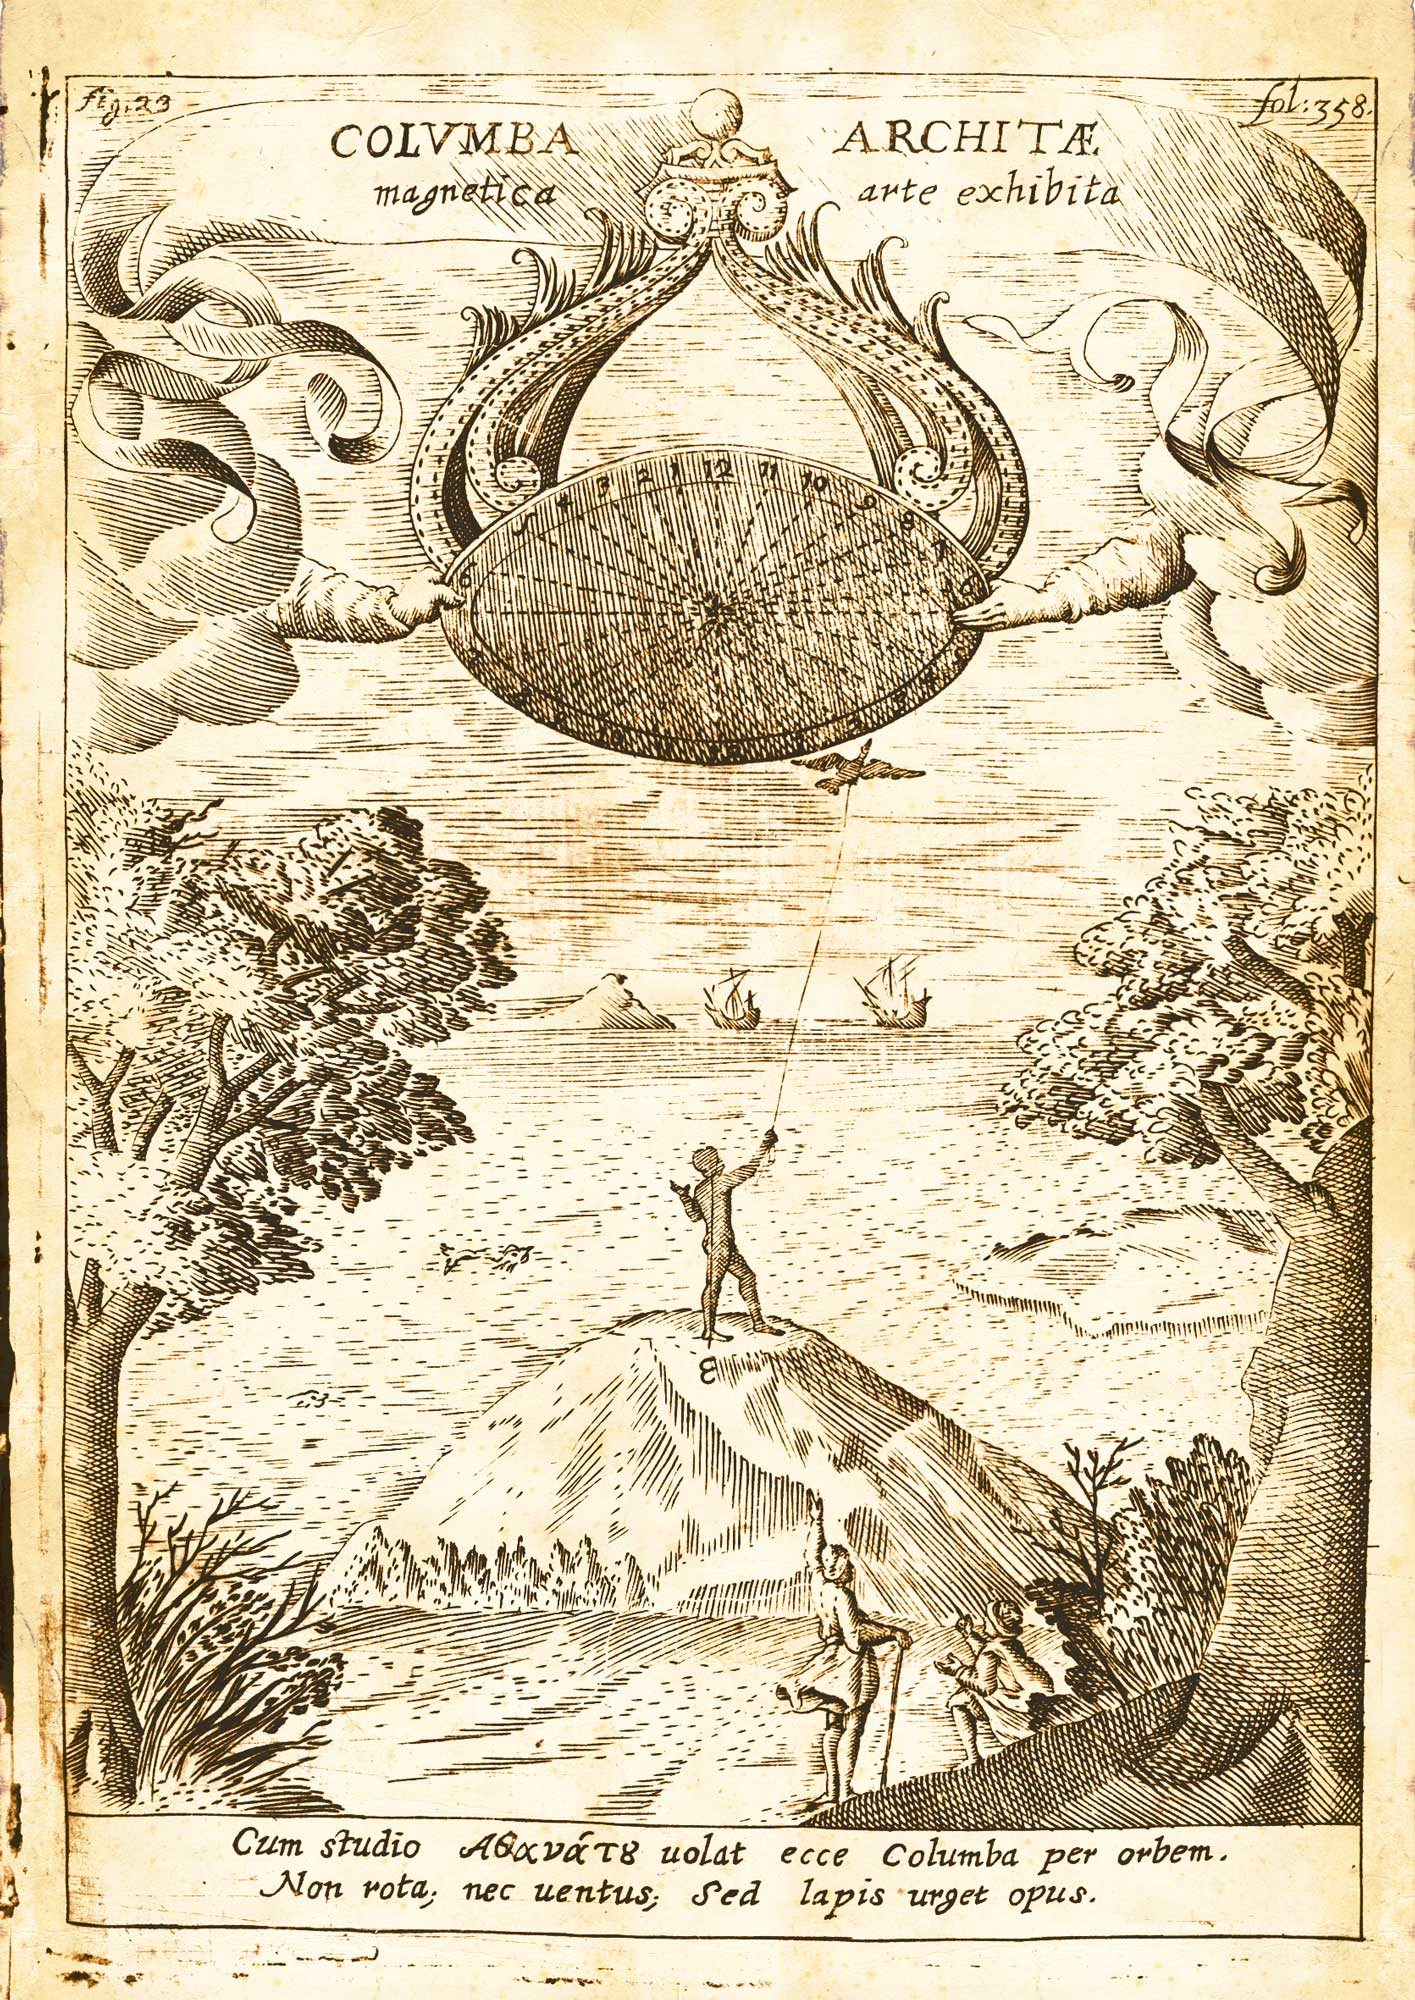
\includegraphics[width=0.5\textwidth]{./EtapaPrimeriza/imagenes/paloma.jpg}
  \caption{Paloma de Arquitas de Tarento}
  \label{paloma}
\end{center}
\end{figure}


\textbf{Apolonio de Pérgamo}, entre 262-190 a.C. , diseñó unos autómatas musicales que funcionaban impulsados por la fuerza del agua.\\


\textbf{Ctesibio de Alejandría}, en el año 300 a.C., también inventó autómatas musicales pero en este caso funcionaban por la impulsión de aire a través de diversos tubos. Pero su contribución más relevante fue el desarrollo del \textit{reloj de agua o clepsidra} que fue el más preciso de los relojes creados hasta la aparición del reloj de péndulo. Este mide el tiempo en función de lo que tarta en caer el agua de un recipiente a otro. Hasta ese momento, el tiempo se medía el tiempo a través de la observación del movimiento del sol, esto permitía medir el tiempo en cualquier momento del día. A continuación se muestra una imagen:\\

	
\begin{figure}[H]
\begin{center}
  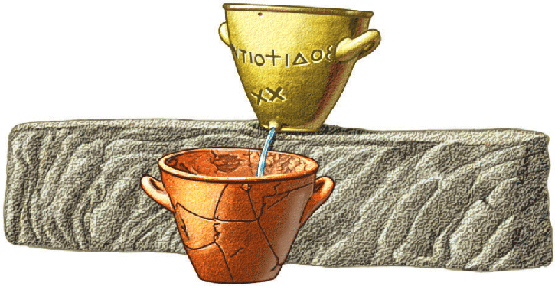
\includegraphics[width=0.5\textwidth]{./EtapaPrimeriza/imagenes/reloj.png}
  \caption{Reloj de Agua de Ctesibio de Alejandría}
  \label{reloj}
\end{center}
\end{figure}



\textbf{Filón de Bizancio} inventa en el año 200 a. C., hizo numerosas contribuciones a la ciencia que se describirán a continuación. Uno de los inventos más revolucionarios fue el molino de agua que se utilizaba tanto para moler grano como para diversos trabajos agrícolas. Además ideó la bomba de agua, esta permitía transportar el agua desde un nacimiento hasta una zona geográficamente más alta mediante la fuerza de la propia agua. Además, relacionado también con el agua, ideó un lavabo en el que, como se puede ver en la siguiente imagen, contenía en su parte superior un recipiente lleno de agua. Esta agua caía sobre un cucharon situado bajo este y cuando este se llenaba se inclinaba y el agua caía sobre el grifo y podía obtener el agua de forma dosificada. Al mismo tiempo que el agua caía por el grifo, también se dejaba caer una pequeña piedra pómez para limpiarte.\\


\begin{figure}[H]
\begin{center}
  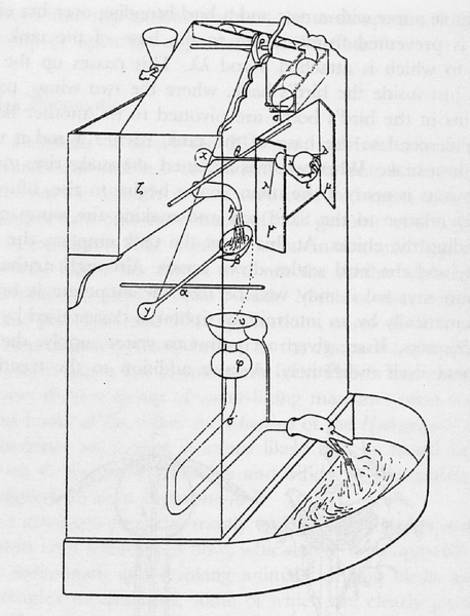
\includegraphics[width=0.3\textwidth]{./EtapaPrimeriza/imagenes/lavabo.jpg}
  \caption{Lavabo de Filón de Bizancio}
  \label{lavabo}
\end{center}
\end{figure}

Pero estas no fueron las únicas contribuciones de Filón de Bizancio. Tenía cierto interés por el tema armamentístico y es por ello que diseñó las primeras flechas, una ballesta que esta compuesta pos dos cadenas unidas con una polea tal que se lanzaban flechas mientras le quedaran en la recámara. Y por último, y uno de sus inventos más curiosos fue lo que se llamó una \textit{camarera automática}. Esto era una estatua que tenía colocado en una de sus manos una jarra y cuando se le colocaba en la otra mano un vaso, esta cedía por el peso y el tubo que conectaba la jarra con el depósito del vino se accionaba para llenar el vaso. 



\textbf{Heron de Alejandría} destaca por las numerosas contribuciones que hizo a la ciencia en la antigüedad. Es por ello que se va a hacer desarrollar sus contribuciones más relevantes y algunas de ellas han facilitado avances industriales a lo largo de la historia.

En sus contribuciones a lo que podría ser la robótica de la época se destaca su trabajo conocido como \textit{Mecánica}, en el que se plasman los primeros datos descriptivos acerca de la construcción de un autómata. Está compuesto por tres libros en los que se trata de las proporciones de las figuras en el primero de ellos, en el segundo de los sistemas mecánicos simples que son descritos en el siguiente apartado y finalmente en su último libro hablaba sobre las aplicaciones de la mecánica.

Cuando hablamos de inventos concretos se destaca que creó la primera máquina de vapor de la historia a la que llamaron \textit{eolípila}. Esta estaba compuesta por una caldera de agua hirviendo y sobre esta se situaba una esfera hueca llena de agua conectadas ambas cosas por dos tubos como se ve en la siguiente imagen\ref{mv}. Cuando el agua hervía se conseguía que la esfera girase a gran velocidad. En la época se dice que solo servía como un divertimento para los niños pero la realidad es que en el futuro serviría como inspiración a las máquinas de vapor utilizadas en las industrias.

\begin{figure}[H]
\begin{center}
  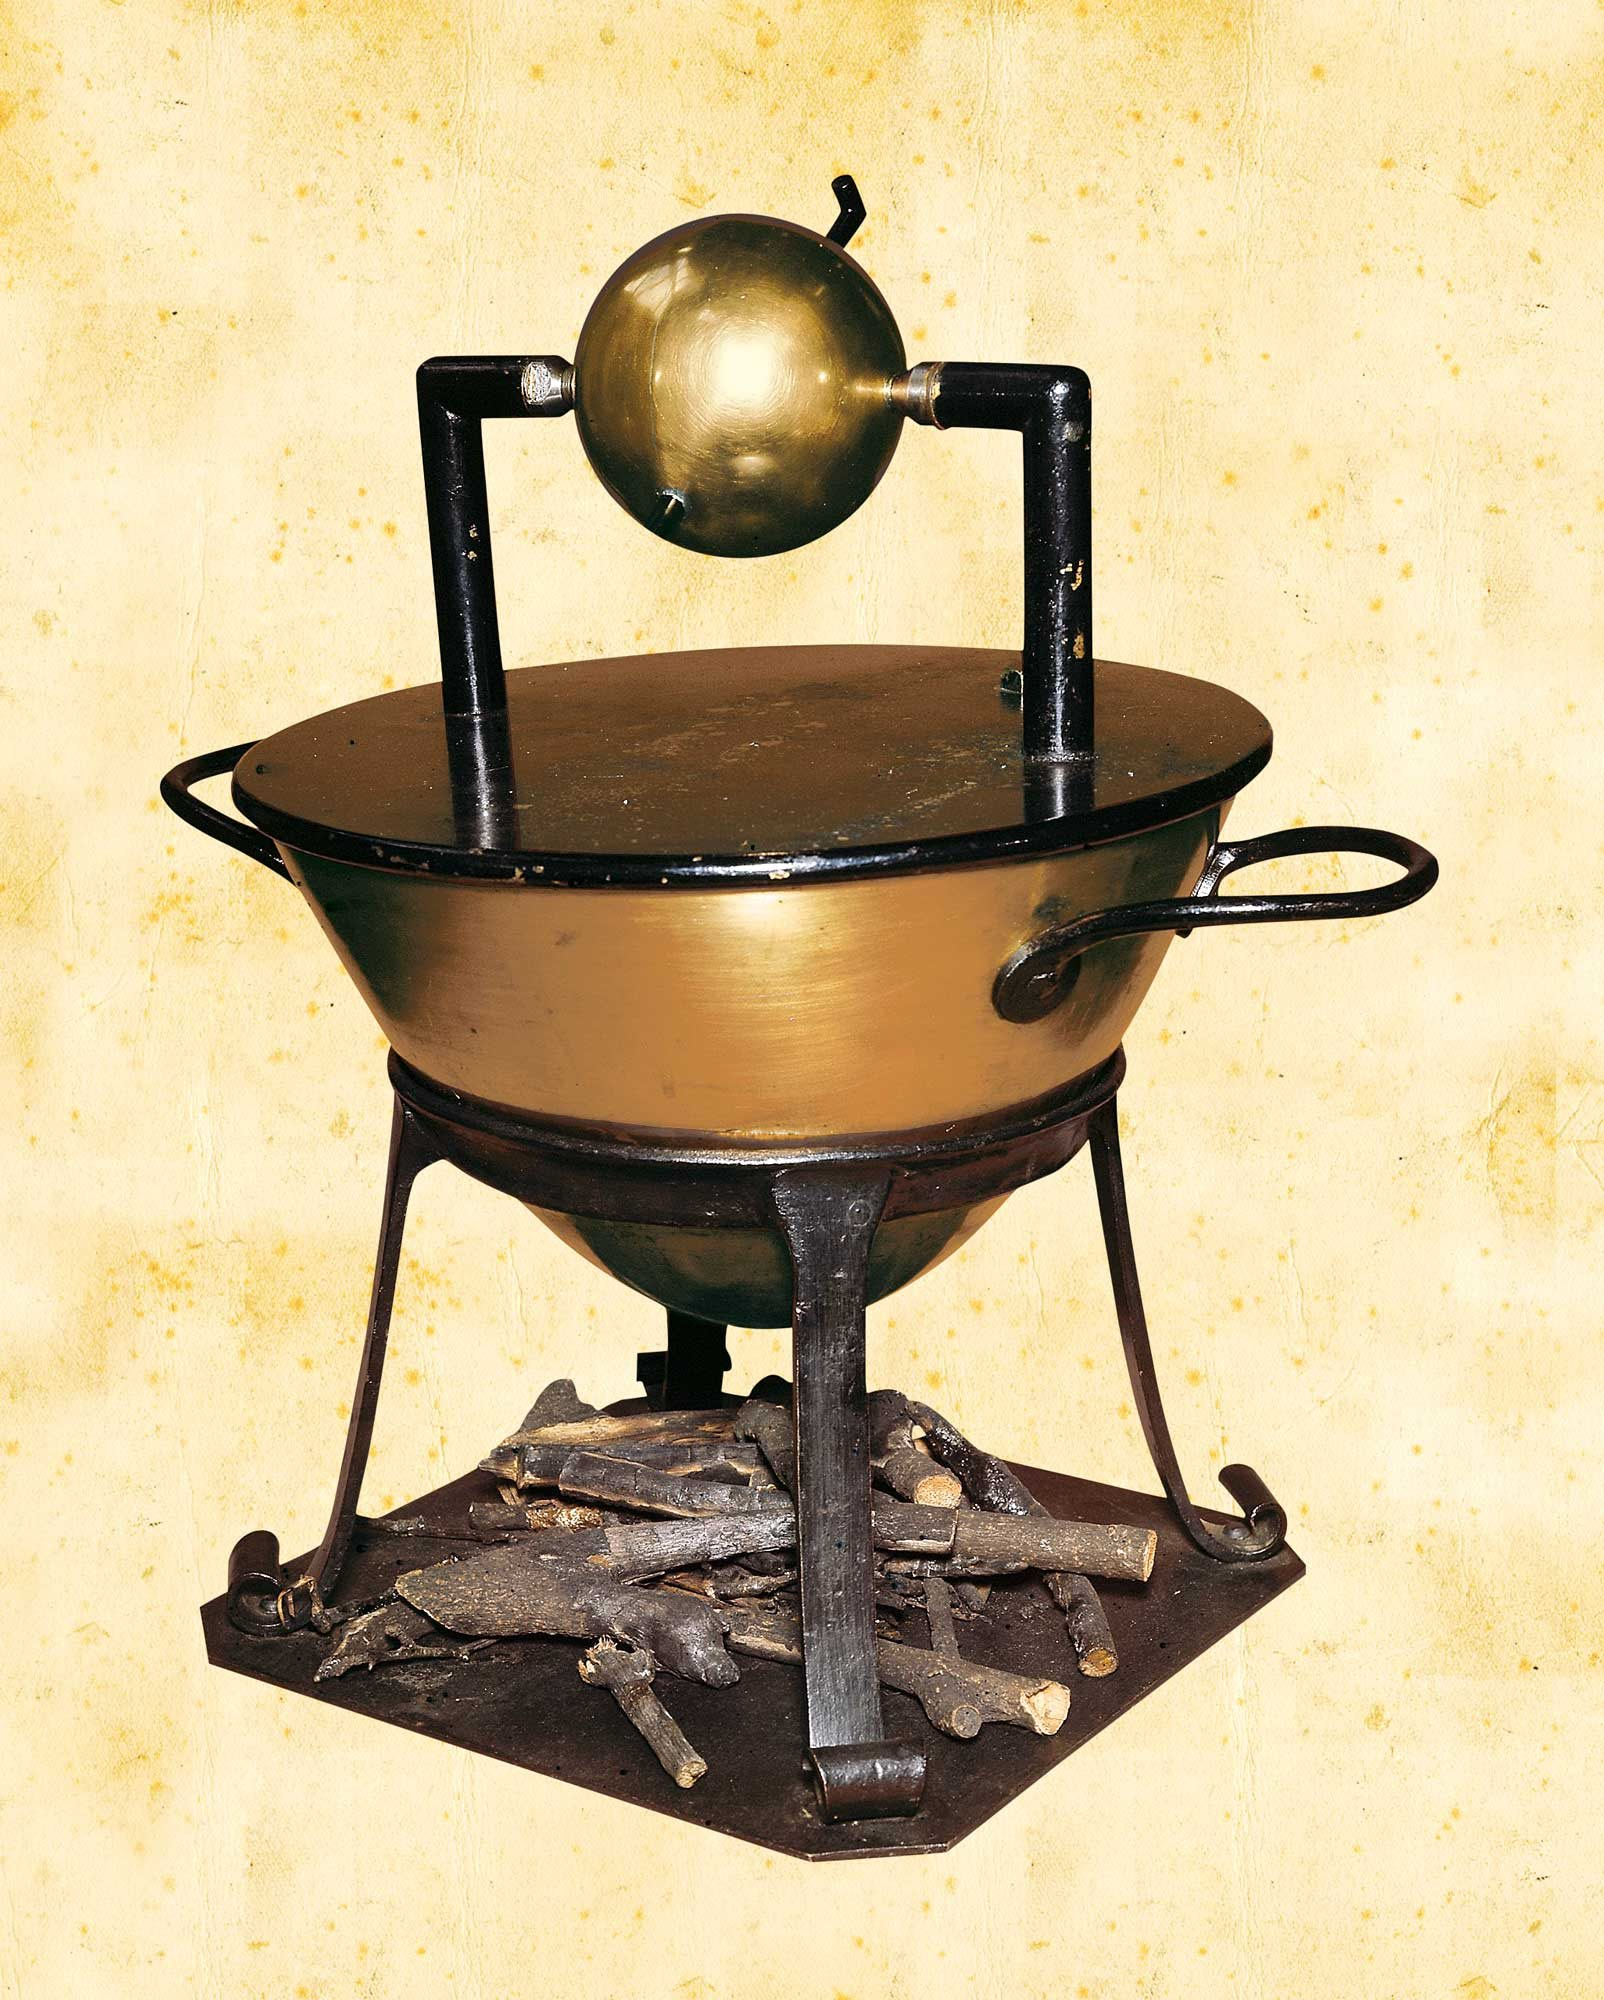
\includegraphics[width=0.3\textwidth]{./EtapaPrimeriza/imagenes/mv.jpg}
  \caption{Eolípila de Heron}
  \label{mv}
\end{center}
\end{figure}

Además diseñó lo que fueron los primeros autómatas y las primeras puertas automáticas. Con la energía que proporcionaba la \textit{eolípila} y con sistemas mecánicos simples como cuerdas, poleas, cadenas y demás era capaz de poner en movimiento autómatas y puertas automáticas. La realidad es que no existe constancia de que lo llevara acaba pero la idea si que la tuvo y dejó constancia de ello en sus libros.


En el 770 d. C., \textbf{Yang Wu-Lien } diseñó un prototipo con forma de mono que alargaba la mano para que le dieran limosna. Cuando la mano alcanzaba un cierto peso, este guarda el dinero en una bolsa.\\



En el 890, \textbf{Han Chih Ho} creó un gato de madera que se encargaba de cazar ratas y ratones que hubiese a su alrededor.\\

El principe hindú \textbf{Bhoja}, en el año 1050, escribió \textit{Samarangana-Sutradhara} donde se describe cómo es el proceso de construcción de máquinas que eran capaces de actuar autonomamente y que se las llamaba yantras.\\

En el siglo XII Al-Jazari (o Al-Djazari)

En la antigüedad, las máquinas más perfectas que se consiguieron fueron los relojes ya que se acercaban al concepto de automatismo y por consiguiente al de robótica. Algunos de ellos cuentan con figuras humanas que sus movimientos van en función del transcurso de las horas. Ejemplos de ello son los relojes de la catedral de Munich y el reloj de Ánker que se puede visitar en la ciudad de Viena, Austria.

Más concretamente, en España se conserva un reloj construido en el siglo XVI, llamado Papamoscas,  y que está compuesto por un hombre que se mueve con los cambios horarios. Hoy en día sigue funcionado y se puede visitar en la catedral de Burgos.

\begin{figure}[H]
\begin{center}
  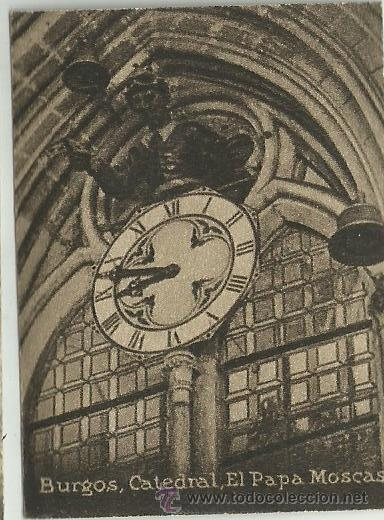
\includegraphics[width=0.3\textwidth]{./EtapaPrimeriza/imagenes/papamoscas.jpg}
  \caption{Papamoscas de la catedral de Burgos}
  \label{papam}
\end{center}
\end{figure}


Aunque se ha de señalar que el robot más antiguo, que estuvo en funcionamiento entre 1352 y 1789, y que se conserva en la actualidad es el Gallo de Estrasburgo. Este formaba era parte del reloj de la catedral de Estrasburgo y hacía mover sus alas y su pico al dar las horas.

\begin{figure}[H]
\begin{center}
  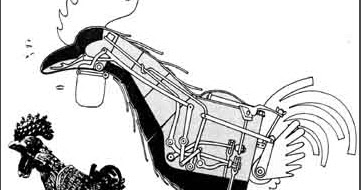
\includegraphics[width=0.3\textwidth]{./EtapaPrimeriza/imagenes/gallo.jpg}
  \caption{Gallo de Estrasburgo}
  \label{gallo}
\end{center}
\end{figure}



Finalmente, para terminar con los orígenes de la robótica no podemos dejar de nombrar "\textit{el hombre de hierro}" de Alberto Magno del siglo XIII. Este era un autómata con forma de humano construido con hierro, cristal y cuero y que era capaz caminar, abrir puertas, entretener invitados y hasta incluso hacer tareas del hogar. Este es considerado como el inicio de lo que hoy en día es la inteligencia artificial.



 

\subsection{Sistemas Mecánicos Simples}

Cuando nos referimos a Sistemas Mecánicos Simples\ref{sms} se hace referencia a aquellos formados principalmente por componentes, dispositivos o elementos que tienen como función transformar o transmitir el movimiento desde las fuentes que los generan al transforman distintos tipos de energía.

A continuación se describen los principales Sistemas Mecánicos Simples:

\begin{itemize}

\item \textbf{La Rueda:} Pieza mecánica circular que rota alrededor de un eje.

\begin{itemize}
\item El Rodillo: Se trata de un cilindro con un diámetro ancho y con una destacada longitud, que al igual que lo hace la rueda, gira alrededor de un eje.

\item Tren de Rodadura
\item Rueda Dentada: Se trata de una rueda cuyo perímetro está totalmente cubierto de dientes. Su ventaja recae en proporcionar movimiento circular mediante el contacto de los dientes entre dos ruedas.

\item Polea Fija: Se trata de una polea en el que la polea se encuentra fija en la parte superior.

\item Polea Móvil: Se trata de una polea conectada a una cuerda en cuyos extremos está, por un lado, anclada a un punto fijo y en otro a un extremo móvil.

\item Polipasto: Conjunto de poleas en la cual una queda fija y la otra tiene movilidad.


\end{itemize}

\item \textbf{La Palanca} 

\begin{itemize}
\item Palanca de Primer Grado: Se trata de una palanca donde el punto de apoyo se sitúa entre la Potencia y la Resistencia. Un ejemplo claro de este tipo de palanca podría ser unas tijeras o una balanza.

\item Palanca de Segundo Grado: Se trata de una palanca en la cual la Resistencia se sitúa entre el punto de apoyo y la fuerza. Un ejemplo de este tipo de palanca podría ser un cascanueces o una carretilla de obra.

\item Palanca de Tercer Grado: Se trata de una palanca en la cual la fuerza se sitúa entre la resistencia y el punto de apoyo. Un ejemplo de este tipo de palanca podría ser un martillo o una caña de pescar.

\end{itemize}

\item \textbf{Plano Inclinado}

\begin{itemize}
\item La Rampa: Superficie plana que forma un ángulo agudo con la superficie.

\item Cuña: Se trata de un prisma triangular que actúa como un plano inclinado móvil.

\item Sistema Tornillo-Tuerca: Sistema en el que un tornillo rota en el interior de una tuerca. Se utiliza para unir de forma no permanente dos elemento.

\item Tirafondo: Tipo de tornillo que tiene una cabeza diseñada para ejercer el giro en esta mediante la ayuda de una herramienta.

\end{itemize}

\end{itemize}

\subsection{Leonardo da Vinci}


Leonardo da Vinci es un artista renacentista conocido principalmente por sus aportaciones en la pintura con son \textit{La Mona Lisa} o \textit{La Última Cena}. Pero este también era arquitecto, botánico, escritor, científico, filósofo, ingeniero e inventor entre otras cosas. Es por ellos que a continuación se va a hablar sobre su importante aportación al ámbito de la robótica.\\

En torno al año 1495, Leonardo da Vinci diseña un autómata con forma de humano que se conoce como \textit{El robot de Leonardo}. Este tenía forma de guerrero medieval y el objetivo de su construcción es la aplicación práctica del estudio sobre el canon de proporciones humanas que se refleja en su obra \textit{El Hombre de Vitruvio}. No se tienen restos en la actualidad de aquel autómata pero si que existen bocetos que nos permiten confirmar su existencia además de permitir probar que funcionaba correctamente. Gracias a dichos bocetos se volvió a construir en el años 2007.\\

Más tarde, en 1515 Leonardo creó un león mecánico que serviría como regalo a la monarquía francesa, concretamente al rey Francisco I, cuando la comunidad florenciana hizo una nueva alianza con Francia. Se trataba de un león de tamaño real y con una gran melena rizada. Este león es capaz de caminar, mover la cabeza, la cola y la boca y lanzar pétalos de flores de lis de uno de sus compartimentos, símbolo este de la monarquía francesa. Este, al igual que ocurrió con el \textit{El robot de Leonardo} ha sido reconstruido recientemente gracias a los bocetos encontrados de la época.


\subsection{Máquina Calculadora de Pascal}

Una de las grandes contribuciones de la ciencia fue el desarrollo de la máquina calculadora. La primera calculadora mecánica de la historia, conocida como Pascalina, fue inventada por el francés \textit{Blaise Pascal}. Fue el joven a la edad de diecinueve años, en 1642, cuando este inventó una máquina que era capaz de realizar sumas, restas hasta incluso multiplicar y dividir mediante restas y sumas sucesivas. Este tuvo una gran repercusión computacional tanto es así que aún sigue teniendo influencia en nuestros días. A continuación se muestra una imagen de dicha calculadora.

\begin{figure}[H]
\begin{center}
  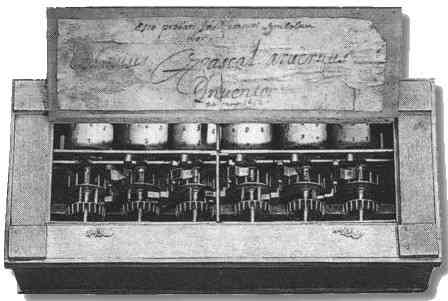
\includegraphics[width=0.4\textwidth]{./EtapaPrimeriza/imagenes/cp.jpg}
  \caption{Calculadora Pascalina}
  \label{cp}
\end{center}
\end{figure}

La máquina estaba compuesta de 8 ruedas dentadas conectadas entre sí con una numeración en ellas de 0 a 9 y una manivela que en función de de la forma de girarla indicaba la operación matemática que se quería realizar. Las 8 ruedas estaban distribuidas de la siguiente manera: dos de ellas se dedicaban a número decimales y las 6 restantes se utilizaban para números enteros. Esto significa que la calculadora te permitía hacer operaciones con número entre 0,01 y 999.999,99 lo que facilitaba un amplio rango de operaciones.\\

Lo curioso recae en el cómo se le ocurrió al joven Pascal inventar la calculadora. Este era hijo de un funcionario recaudador de impuesto y en numerosas ocasiones ayudaba a su padre a redactar informes oficiales. Pascal pensó que si conseguía crear una calculadora ahorraría mucho tiempo y al mismo tiempo se aseguraba que los resultados eran correctos. Como resultado de ello apareció la primera calculadora mecánica de la historia dejando atrás instrumentos para contar como puede ser el ábaco.





\subsection{Isaac Asimov y las reglas de la robótica}

Isaac Asimov nacido en 1920 en la ciudad de Petrovichi, RSFS de Rusia. Con apenas tres años de edad su familia se trasladó a los EE.UU. y fue allí donde desarrolló su vida familiar, académica y laboral. A modo de curiosidad, señalar que debido a su precocidad intelectual sus padres decidieron falsificar su fecha de nacimiento para ingresar antes en un colegio neoyorkino. Una vez en la universidad se licenció e Químicas, Ciencias y Artes, Bioquímica y se doctoró en Filosofía. A lo largo de su vida tuvo dos esposas pero en ningún caso descendencia. Finalmente en 1992 fallece en Nueva York a causa del sida que había contraído en una transfusión sanguínea.\\

Durante su vida, Asimov destacó como escritor de ciencia-ficción y de divulgación científica. Fue en su libro \textit{"Yo robot"} donde este aventuró la relación que tendríamos los humanos con los robots, pero claro dichos robots no garantizaban la seguridad y prevención total de los riesgos. Es por ello que Asimov estableció las tres siguientes reglas de la robótica:

\begin{enumerate}
\item Un robot no hará daño a un ser humano o, por inacción, permitirá que un ser humano sufra daño.
\item Un robot debe cumplir las órdenes dadas por los seres humanos, a excepción de aquellas que entrasen en conflicto con la primera ley
\item Un robot debe proteger su propia existencia en la medida en que esta protección no entre en conflicto con la primera o con la segunda ley
\end{enumerate}

Señalar que Isaac Asimov era un adelantado a su tiempo y es que apostaba por la divulgación científica a través de la red. Es por ello que en 1988 aventuró la existencia de una plataforma como Wikipedia 13 años antes de que esta existiera. Además afirmaba la existencia en el futuro de plataformas como Skype, FameTime o el desarrollo de coches autónomos lo que hoy en día es una realidad.



\subsection{Tortugas autónomas de Walter}

William Grey Walter nació en Kansas (EE.UU.) en 1910 y se trata de uno de los pioneros en el campo de la robótica, cibernética e inteligencia artificial. Sus estudios en neurología le llevaron a la investigación y desarrollo inventos que eran capaces de medir ondas cerebrales y analizar el comportamiento del cerebro de una persona. Más concretamente, con la idea que que la conexión de neuronas o células cerebrales se podían ejecutar comportamientos complejos. Esto dio lugar a la construcción en 1948 y 1949 de las \textit{tortugas} Elmer y Elsie, respectivamente. En la siguiente imagen se pueden observar como eran estas.

\begin{figure}[H]
\begin{center}
  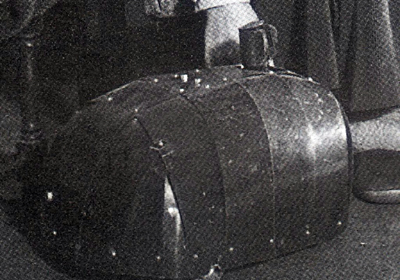
\includegraphics[width=0.5\textwidth]{./EtapaPrimeriza/imagenes/tortuga.jpg}
  \caption{Tortuga autónomas de Walter}
  \label{tortuga}
\end{center}
\end{figure}

El nombre de tortugas se debe al caparazón de plástico que protegía al robot además de su lentitud en los movimientos. Estas solo estaban programadas para hacer dos misiones como son esquivar obstáculos aunque no de una forma muy inteligente y volver a recargar su batería cuando esta estuviera cerca de agotarse. Este estaba formado por tres ruedas, una batería y una célula fotoeléctrica móvil que actuaba sobre el motor para decidir la dirección de los movimientos como lo hacen los actuales sensores.

\begin{figure}[H]
\begin{center}
  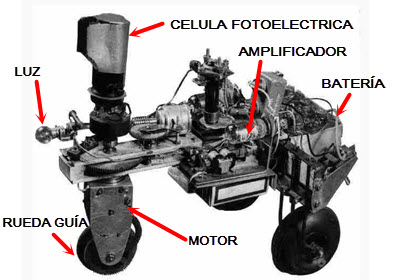
\includegraphics[width=0.5\textwidth]{./EtapaPrimeriza/imagenes/t1.jpg}
  \caption{Estructura de las Tortuga autónomas}
  \label{t1}
\end{center}
\end{figure}


Walter fue el precursor de los robot aspiradores están tan de moda en nuestros días y que nos facilitan notablemente las tareas del hogar.


\subsection{El brazo robótico teleoperado de Goertz}


El primer brazo mecánico teleoperado se desarrollo por Raymond Goertz en 1949 y fue llamado \textit{M1}. El objetivo de su desarrollo era proteger del riesgo a los trabajadores mientras se permite la manipulación precisa de materiales o elementos radiactivos. Este es considerado el pionero en aplicar la técnica maestro-esclavo en sistemas de teleoperación. Más concretamente, en la máquina se consideran dos dispositivos diferenciados un brazo \textit{maestro} y otro brazo \textit{esclavo}. El brazo \textit{esclavo} se ubica dentro de un recipiente aislado en su totalidad y el brazo \textit{maestro} se sitúa en una sala de control y es el encargado de ejecutar ordenes que posteriormente el \textit{esclavo} reproducirá sobre el material radioactivo con notable precisión.

En 1951, Goertz diseñó una mejora en este brazo mediante la incorporación de una serie de poleas y cables de acero entre el brazo \textit{maestro} y el brazo \textit{esclavo} que proporcionaba mayor precisión en sus movimientos.\\

Durante el desarrollo de dicho brazo robótico, Goertz estableció uno principios que debía cumplir un brazo de este tipo y que aun se siguen aplicando a los robots quirúrgicos que se utilizan hoy en día. Los principios son los siguientes:

\begin{enumerate}
\item El movimiento del brazo \textit{esclavo} debe tener seis grados de libertad; tres de traslación, tres de rotación y uno de agarre.

\item El movimiento del brazo \textit{esclavo} debe estar acoplado al brazo \textit{maestro}.

\item Dicho acoplamiento debe ser bilateral, es decir, las fuerzas sobre el brazo \textit{esclavo} deben reflejarse en el brazo \textit{maestro} y los desplazamientos de producidos por el brazo \textit{maestro} deben producir el mismo desplazamiento sobre el brazo \textit{esclavo}.

\end{enumerate}


Seguidamente se muestra una imagen donde se puede observar el brazo robótico de Goertz descrito anteriormente.



\begin{figure}[H]
\begin{center}
  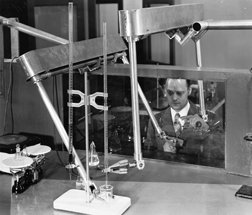
\includegraphics[width=0.5\textwidth]{./EtapaPrimeriza/imagenes/brazo.jpg}
  \caption{Brazo robótico de Goertz}
  \label{brazo}
\end{center}
\end{figure}


\subsection{Autónoma Universal de George Devol}

\textbf{George Devol} es conocido como el creador del primer robot industrial además de cofundador de la primera empresa robótica de la historia llamada \textit{\textbf{Unimation}} junto al empresario  Joseph F. Engelberger.

Este tenía el objetivo de crear una máquina que fuese fácilmente manejable y que trabajara de forma automática. Fue en el año 1948 cuando Devol patentó el prototipo de lo que más tarde se convertiría el primer robot de uso industrial. Este robot era un brazo que tenía la función de mover artículos de gran tamaño y gran peso en el ámbito industrial. Además era capaz de mover piezas a altísimas temperaturas y de hasta 225 kilos de peso.

Señalar que Devol y  Engelberger formaban un tándem perfecto, uno aportaba sus cualidades creativa y el otro las suyas empresariales. Esto les permitió fundar lo que fue la primera empresa robótica de la historia además de conseguir un contrato con la empresa \textit{Generals Motors} para instalar el brazo robótico en su fábrica de Nueva Jersey. Poco después, en 1968, firmó un contrato similar con la empresa japonesa de \textit{Kawasaki}. Señalar que en esa época las dos potencias industriales mundiales eran Japón y Estados Unidos y que por el contrario en Europa este tema estaba más estancado.

Más tarde, en 1978, Devol consigue mejorar este brazo robótico haciendolo programable y multiarticulado, lo que permitía colocar las piezas en cualquier posición que se quisiese siempre que estuviese a su alcance. Este fue llamado \textbf{\textit{PUMA}} (\textit{Programmable Universal Machine for Assembly}).

Señalar que George Devol murió en 2011 a los 99 años de edad y que no se le puede negar la gran aportación a la industria que ha realizado ya que puso la primera piedra de la industrias robotizadas de la actualidad.






\subsection{Sputnik}

El programa \textbf{Sputnik} se trataba de una serie de misiones espaciales ejecutadas por la antigua Unión Soviética a finales de los años 50 y principios de los 60 del siglo pasado. El objetivo de este programa era probar la viabilidad de los satélites artificiales alrededor de la órbita de nuestro planeta.
Como curiosidad, señalar que el origen de la palabra \textit{Sputnik} proviene del ruso y significa \textit{satélite} o \textit{compañero de viaje}.
Durante este programa se lanzaron al espacio hasta 10 satélites diferentes. Seguidamente se describirán cada uno de ellos y el impacto que esto tuvo.\\


\textbf{Sputnik 1}\ref{s1} fue el primer satélite artificial de la historia el cual fue lanzado el 4 de Octubre de 1957. La importancia de este satélite recae en que fue el primer intento sin fallo de poner a orbitar alrededor de nuestro planeta un satélite artificial. Fue lanzado con el lanzador R-7 y este se encargó de analizar señales de radio que utilizaba para conocer la cantidad de electrones en la ionosfera. Estuvo en actividad durante 92 días y en la actualidad se puede visitar en la oficina neoyorkina de las Naciones Unidad.\\ 

\begin{figure}[H]
\begin{center}
  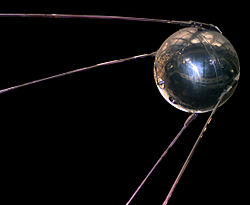
\includegraphics[width=0.5\textwidth]{./EtapaPrimeriza/imagenes/s1.jpg}
  \caption{Sputnik 1}
  \label{s1}
\end{center}
\end{figure}

Más tarde, se lanzó el \textbf{Sputnik 2}\ref{s2} el 3 de Noviembre de 1957. A diferencia del \textit{Sputnik 1}, este portaba un ser vivo en su interior. Aquí viajó la conocida \textit{Perra Laika}, y el objetivo de este lanzamiento era comprobar el efecto que causaba el medio espacial en un ser vivo. Regresó a La Tierra tras 162 días de actividad y en aquel momento de publicó que \textit{Laika} murió al regreso a nuestro planeta. Sin embargo, en 2002 fuentes rusas declararon que el animal había muerto al poco tiempo de ser lanzada a causa del estrés y el sobrecalentamiento del satélite.\\

\begin{figure}[H]
\begin{center}
  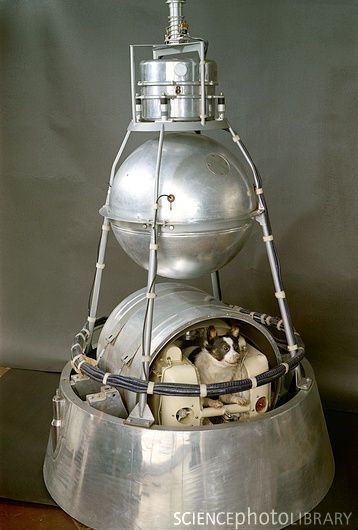
\includegraphics[width=0.3\textwidth]{./EtapaPrimeriza/imagenes/s2.jpg}
  \caption{Sputnik 2 con Laika en su interior}
  \label{s2}
\end{center}
\end{figure}

Fue el 3 de Febrero de 1958 cuando se intento lanzar el siguiente satélite, \textbf{Sputnik 3}. Esto quedó en un solo intento ya que fue fallido. Pero más tarde, se consiguió volver a lanzar esta vez ya correctamente. A pesar de que el sistema de grabación falló, transportó instrumentos para explorar la atmósfera superior y el espacio próximo.\\

\textbf{Sputnik 4} que fue lanzado el 15 de Mayo de 1960, fue el primer prototipo de nave espacial lanzada desde nuestro planeta y llevaba a bordo un maniquí de un hombre, un sistema de televisión y una cabina de soporte biológico. Pero un fallo en el sistema de guía la reubicó en una órbita más alta a la terrestre. Regresó el 5 de Septiembre de 1962, pero nada más tomar contacto con la atmósfera terrestre se desintegró. Algunas de sus piezas fueron encontradas al norte de los Estados Unidos, en Wisconsin.\\

Más tarde, el \textbf{Sputnik 5} se lanzó el 19 de agosto de 1960 y esta llevaba a bordo a los perros \textit{Belka} y \textit{Strelka} además de 40 ratones y numerosas plantas. La nave solamente permaneció en el espacio un día y todos los seres vivos regresaron con vida.\\

\textbf{Sputnik 6} fue enviado al espacio el 1 de Diciembre de 1960 con los perros \textit{Pchelka} y \textit{Mushka} junto a una serie de insectos, animales y plantas, y la cápsula no se consiguió recuperar. \\

Más tarde, el 4 de Febrero de 1961, \textbf{Sputnik 7} fue el primer intento de exploración de Venus. Sin embargo, el sistema de ignición tuvo un fallo y la sonda regresó a la órbita terrestre en lugar de tomar dirección a Venus.\\

Seguidamente, \textbf{Sputnik 8} se envió el 12 de Febrero de 1961 que transportaba la sonda Verena 1. Esta fue la primera nave espacial lanzada para sobrevolar el planeta Venus.\\

\textbf{Sputnik 9} fue una de las pruebas que tenían como finalidad precursar los vuelos espaciales tripulados por humanos. Este completó un giro completo alrededor de nuestro planeta y volvió sin ningún problema lo que supuso un gran éxito.\\

Finalmente el \textbf{Sputnik 10}, al igual que el \textbf{Sputnik 9}, se trataba de una serie de pruebas con naves espaciales diseñadas para tripulación humana. Este portaba un perro, un astronauta ficticio y un sistema de televisión. Al igual que el anterior, se recuperó con éxito.

\begin{figure}[H]
\begin{center}
  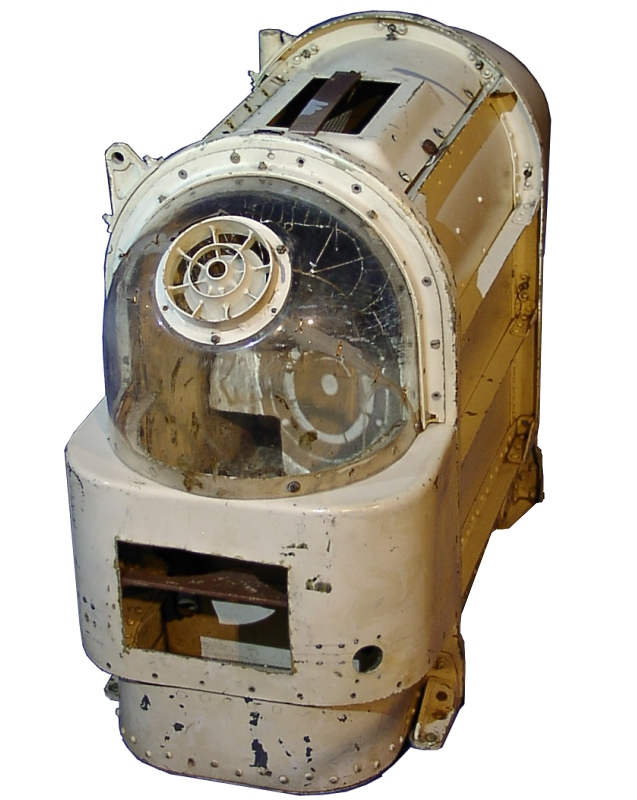
\includegraphics[width=0.3\textwidth]{./EtapaPrimeriza/imagenes/s10.jpg}
  \caption{Sputnik 10}
  \label{s2}
\end{center}
\end{figure}





\subsection{Robots Industriales de Generals Motors}


Por último, como fin a la etapa primeriza de la historia de la robótica vamos a hablar sobre \textbf{General Motors}, empresa norteamericana que destaca como fabricante mundial de vehículos. En 1957 se ofrece a esta empresa el conocido como Controlador Digital Modular, que está compuesto por máquinas de estado secuencial y que trabajan con procesadores centrales con desplazamiento de bits, que es el principio de lo que hoy conocemos como sistemas de control automático.\\


Pero sin duda el hito de \textit{General Motors} fue instalar el primer robot industrial de la historia en sus instalaciones de Trenton, Nueva Jersey, en el año 1960. Este robot era un brazo robótico de 1800 kg de peso y que tenía la función de mover y colocar piezas metálicas de gran tamaño a grandes temperaturas. Señalar que este robot fue comprado a la empresa \textit{\textbf{Unimation}}, que como se ha comentado en apartados anteriores fue la primera empresa robótica de la historia fundada por  George Devol y el empresario  Joseph F. Engelberger.

Es en el 1978 cuando el robot \textit{PUMA}, desarrollado por la empresa de Devol y Engelberger, fue instalado en \textit{General Motors} para realizar tareas de montaje.






\section{Historia Moderna de la Robótica}

%Introducción
\subsection{Introducción}
Acabamos de ver cómo fueron los comienzos de la historia de la robótica desde la época griega hasta los primeros robots industriales de la década de los 60. De aquí en adelante podemos considerar que entramos en la etapa más cercana a nuestros años con un hecho significativo que comenzaremos explicando y marca una diferencia con la etapa previa: la introducción concienzuda de la inteligencia artificial.

\vspace{10px}

Este salto de época viene marcado por la apertura del SRI (Stanford Research Institute) que comienza con la investigación en el campo de la inteligencia artificial tanto en la universidad de Stanford como en la de Edimburgo. Este hecho delimita la historia de la robótica pues es a partir de aquí cuando los investigadores comienzan a dar autonomía e inteligencia a los robots que se pretenden diseñar. Esta herramienta será fundamental en el entendimiento del desarrollo de los robots y las capacidades de los mismos.

\vspace{10px}

De aquí en adelante veremos como los robots han avanzado en una variedad inmensa de campos, incluyendo la movilidad, los brazos robóticos, los sistemas de reconocimiento del entorno y la interacción de los mismos. Actualmente a nadie se le escapa el hecho de que la robótica es una industria que se encuentra en pleno auge y que se prevee que continúe creciendo.

\vspace{10px}

En las secciones posteriores de este trabajo veremos como la robótica ha llegado hasta el momento más actual con aplicaciones como la industria militar, las investigaciones espaciales, las interfaces conversaciones o los robots humanoides, actualmente colocados en el ojo de mira de toda la prensa mundial.


%Desarrollo de los laboratorios de IA
\subsection{Inicios de la Inteligencia Artificial}
\subsubsection{SRI}
SRI o Stanford Research Institute fue una institución amparada bajo la Universidad de Stanford de propósito general en un inicio. Su fundación fue difícil y no fue hasta el tercer intento cuando se consiguió en el año 1946.

\vspace{10px}

El SRI hizo investigaciones en campos muy variados como la agricultura, el ejército o la contaminación pero no fue hasta 1966 cuando se fundó el Centro de Inteligencia Artificial comenzando a funcionar bajo el mando de Charles Rosen. El primer proyecto realizado por el SRI en Inteligencia Artificial fue el Robot Shakey, el primer robot cuya intención no era sólo moverse, si no razonar. Este robot era capaz de analizar el entorno mediante una cámara y procesaba el lenguaje natural para recibir instrucciones. Desarrollando las habilidades de este robot en el desplazamiento, se consiguió que se moviera por una habitación esquivando los obstáculos que se le imponían en la misma. En el SRI se desarrollaron algoritmos de Visión por Computador tales como filtros y convoluciones para detección de bordes de objetos a ser esquivados y además se desarrollaron algoritmos tan importantes como el A*, el algoritmo por excelencia de cálculo de caminos eficientes.

\vspace{10px}

Shakey fue dado por finalizado en el año 1972, siendo ahora los esfuerzos del SRI dirigidos en la creación de Internet para suceder a ARPANET. La primera conexión que se produjo entre dos ordenadores usando Internet como lo conocemos ahora se produjo en 1977 entre los laboratorios del SRI y la universidad de California UCLA.

\vspace{10px}

Tras estos grandes hitos el SRI se desprendió de la Universidad de Stanford para comenzar su andadura como una empresa, fundándose en ese momento la compañía SRI International, pero la Inteligencia Artificial ya había comenzado.

\subsubsection{Laboratorios de IA del MIT}
En la misma época el Instituto Tecnológico de Massachusetts o MIT abrió sus laboratorios de Inteligencia Artificial donde surgieron algunas de las figuras más reconocidas en el ámbito de la computación.

\vspace{10px}

El inicio de la investigación en el ámbito de la computación en el MIT comenzó con figuras tan reseñables como Shannon o Vannevar Bush, el ideólogo del analizador diferencial. En sus comienzos el laboratorio no empezó formándose como tal, si no que se creó un proyecto llamado MAC (Man and Computer) en el que estaban figuras tan importantes como John McCarthy el inventor de Lisp. En un principio el proyecto se dirigió intentando abarcar un amplio rango de temas, como son: la visión por computador, el movimiento mecánico y la manipulación de objetos a partir de máquinas y el manejo del lenguaje natural.

\vspace{10px}
De los despachos en los cuales se llevaban a cabo estas investigaciones surgieron otras figuras como Richard Stallman (creador del proyecto GNU) e invenciones como las máquinas Lisp (máquinas que ejecutaban muy eficientemente Lisp).


%Robotics Institute
\subsection{Robotics Institute}
La Inteligencia Artificial y el desarrollo de la electrónica fue dando paso cada vez con mas fuerza a una nueva rama de la computación: la robótica.

\vspace{10px}

Esta rama es completamente transversal, puesto que aglomera a todos los departamentos relacionados con la computación desde hardware a diseño de software pasando por la visión por computador o la Inteligencia Artificial. Sobre el año 1979 la Universidad Carnegie Mellon en Pittsburgh se dio cuenta del potencial desarrollo de la robótica en un futuro, por lo que decidió abrir un nuevo departamento en la misma que llamó Robotics Institute o Instituto de Robótica, siendo la primera Universidad en tener un departamento dedicado únicamente a la robótica.

\vspace{10px}

Dos robots que podemos destacar de este instituto fueron los vehículos Sandstorm y Highlander dos vehículos completamente autónomos diseñados para realizar un rallie por un desierto llegando entre puntos del mismo sin ninguna intervención humana. Actualmente los avances logrados en la implementación de estos dos vehículos están siendo implementados por las marcas de coches para intentar lograr cada vez una mayor independencia de los conductores de los mismos.

\vspace{10px}

Actualmente el Robotics Institute ya no es sólo un departamento de la Universidad Carnegie Mellon, sino una compañía en si misma con un presupuesto de unos 65 millones de dólares anuales. Algunos de los campos de trabajo en los que se centran son: robots relacionados con la agricultura, robots industriales, robots médicos, robots asistentes y robots relacionados con el transporte de personas y mercancías.


%WABOT
\subsection{El primer robot antropomórfico: WABOT}
Hasta este momentos los robots habían sido proyectos que implementaban funcionalidades concretas tales como moverse, ver, intentar hablar, reemplazar a los humanos en algunas tareas repetitivas, etc.

\vspace{10px}

En la Universidad de Waseda en Japón, se creó el primer robot con forma antropomórfica llamado WABOT 1. Según los integrantes del proyecto si quisieramos que un robot nos ayudase como un asistente sería conveniente que tuviera forma antropomórfica para que nos resultase más familiar, por lo que se plantearon crear un robot asistente inteligente con forma humana. En este proyecto se desarrollaron dos versiones del mismo robot el primero llamado WABOT 1 y tras este crearon WABOT 2.

\vspace{10px}

WABOT 1 fue creado entre los años 1970 y 1973 siendo el primer robot antropomórfico del mundo. El robot tenía control de sus brazos, incorporaba un sistema de visión y análisis del entorno y un sistema conversacional. Éste era capaz de medir su posición con respecto a objetos de la sala y medir las distancias hasta ellos. Además era capaz de andar y coger objetos. En aquel momento, al ser el robot capaz de hablar, se le realizó un test psicológico obteniendo como resultado que WABOT 1 se podría equiparar a un niño de un año de edad.

\vspace{10px}

Tras el éxito del proyecto el grupo de investigación pensó en desarrollar una nueva versión que llamaron WABOT 2 entre los años 1980 y 1984. Esta versión se convirtió en algo mucho menos útil y versátil que WABOT 1, ya que fue diseñado únicamente con el objetivo de que fuera capaz de tocar el piano. Según los propios investigadores esto era interesante pues las artes requieren pensar como un humano y destreza en el movimiento.

\vspace{10px}

Estos dos robots sentaron un precedente abriendo el campo de los robots antropomórficos, los cuales analizaremos en etapas posteriores más cercanas a nuestra época.


%Brazos robóticos
\subsection{Brazos Robóticos}
\subsubsection{Stanford Arm}

Los brazos robóticos han sido un gran pilar en el desarrollo de la tecnología por su gran utilidad. Actualmente rara es la fábrica que no emplea brazos robóticos para hacer la producción mucho más ágil e incluso segura para los operadores de la misma. Este camino fue iniciado en el año 1969 en la Universidad de Stanford por Victor Scheinman.

\vspace{10px}

El primer brazo robótico fue desarrollado bajo el proyecto Hand-Eye en los laboratorios de Inteligencia Artificial de la Universidad de Stanford. El Stanford Arm fue diseñado tras los intentos de hacer brazos operables mediante un humano desempeñados en dicha Universidad. Los intentos precedentes incluían modificaciones de brazos ortopédicos e incluso un modelo hidráulico que resultaba muy peligroso por la rapidez de sus movimientos. El Stanford Arm se creó sin tener una forma antropomórfica y con 6 grados de libertad manipulado de forma completamente eléctrica.

\vspace{10px}

El robot estaba controlado mediante cámaras y elementos parecidos a joysticks gracias a que el brazo llevaba incorporados potenciómetros y sensores que permitían el control del mismo.

\begin{figure}[!h]
	\centering
	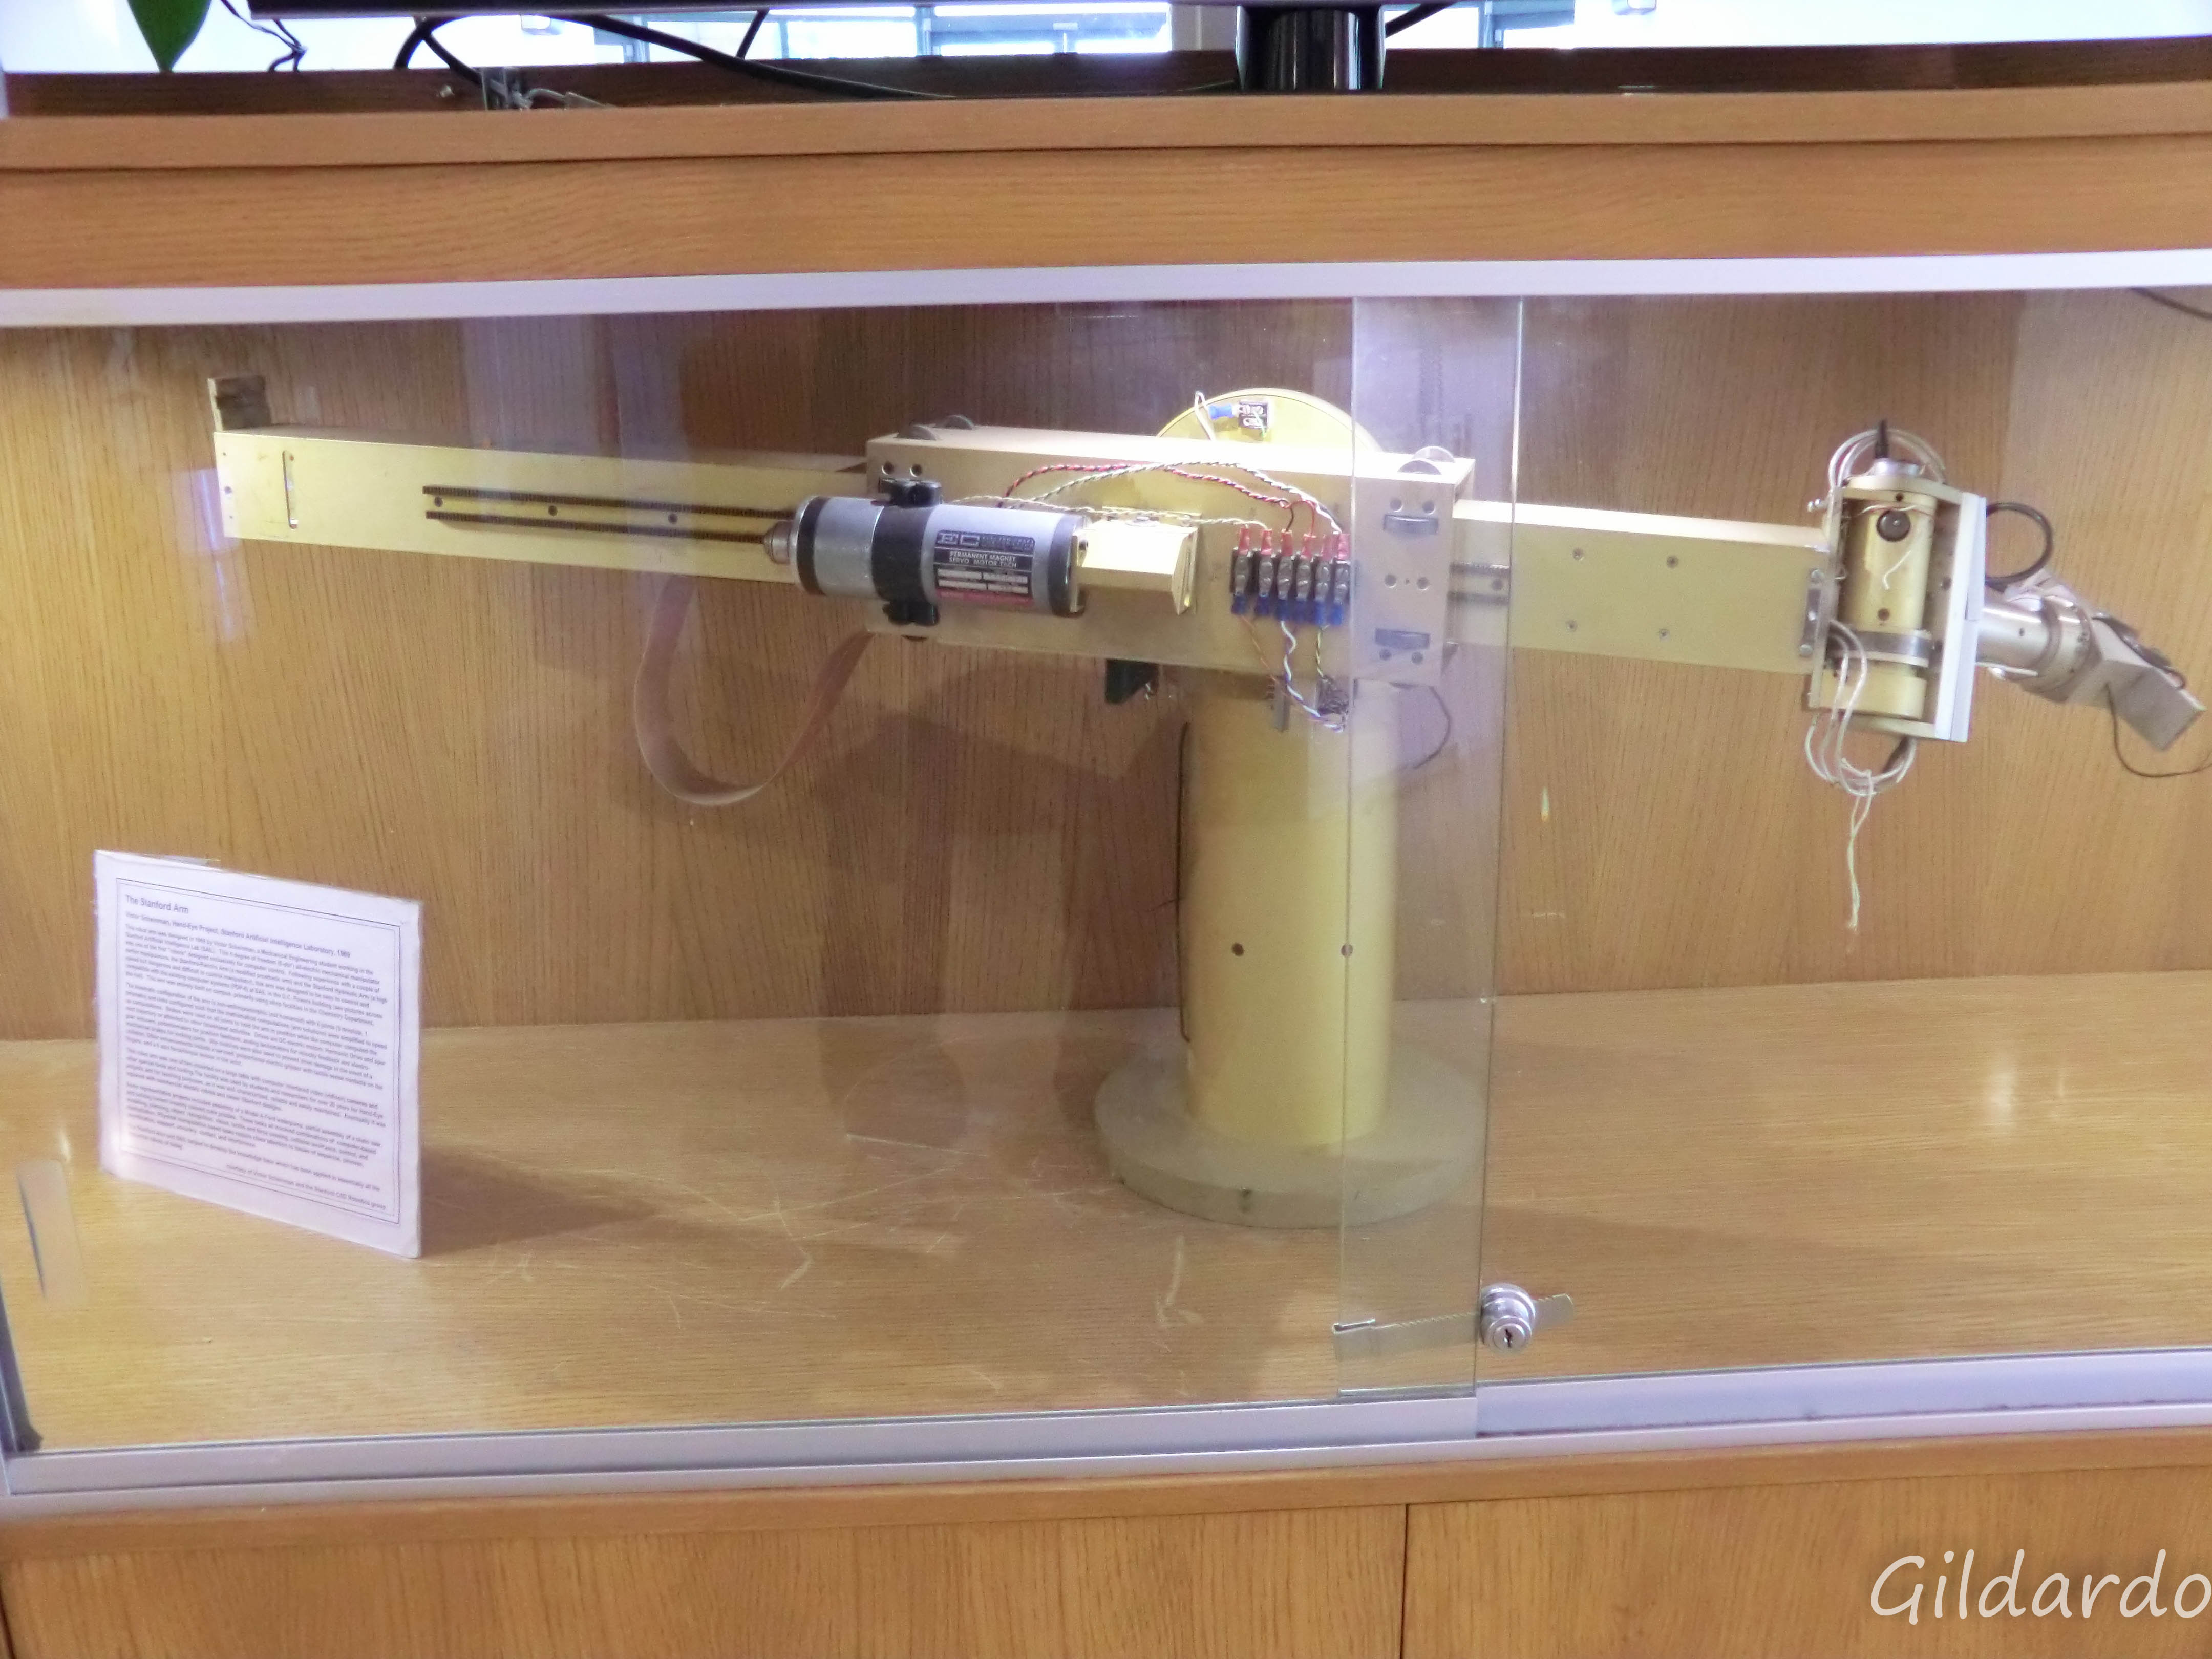
\includegraphics[scale=0.3]{./EtapaModerna/Imagenes/stanford_arm.jpg}
	\caption{Stanford Arm (\href{https://www.flickr.com/photos/gildardo/6186967797}{Flickr})}
	\label{fig:stanfordArm}
\end{figure}

\subsubsection{T3}

Tras los grandes avances del Stanford Arm la compañía Cincinnati Milacron Corp. decidió desarrollar en 1973 el primer brazo robótico pensado para ser incorporado dentro del mercado industrial. El encargado dentro de la compañía de elaborar el diseño del brazo fue Richard Hohn.

\vspace{10px}

Este brazo robótico, al igual que el Stanford Arm fue desarrollado con 6 grados de libertad permitiendo un amplio abanico de movimientos que el brazo podía hacer con bastante precisión.

\vspace{10px}

Este brazo ya no tenía que ser controlado directamente por un humano, si no que implementaba un módulo de decisiones y sensores capaz de saber si había completado una cierta tarea y tenía que realizar algún movimiento, por ejemplo coger un elemento de una cinta de transporte y moverlo.

\subsubsection{PUMA}

Tras el éxito de los diseños de Victor Scheinman en la Universidad de Stanford, la compañía General Motors se interesó en sus prototipos de brazos robóticos. Ante el incipiente mercado de estos robots las grandes compañías con un gran nivel de fábricas comenzaron a ver una utilidad en estos brazos, por lo que General Motors financió a Scheinman para que desarrollara el brazo robótico PUMA (Programmable Universal Machine for Assembly o Programmable Universal Manipulation Arm).

El brazo se comercializó en tres tamaños distintos con la intención de que unos levantasen más peso que otros. Todos los brazos tenían el mismo diseño y los mismos grados de libertad, por lo que los movimientos posibles eran iguales para todos los modelos. Los ángulos máximos de giro y rotación variaban entre modelos, ya que hay que pensar que estos fueron creados casi \textit{ad hoc} para las compañías. Además los modelos más grandes tenían unos movimientos mucho más lentos debido al peso que tenían que soportar y mover por el diseño tan grande que tenían para la época.

Este modelo fue fabricado por General Motors, Westinghouse Electric Corp., Staubli e incluso la división de robótica de Nokia. Fue un éxito fabricándose únicamente por Nokia unos 1500 brazos robóticos PUMA.

\begin{figure}[!h]
	\centering
	\includegraphics[scale=0.3]{./EtapaModerna/Imagenes/puma.jpg}
	\caption{PUMA (\href{https://es.m.wikipedia.org/wiki/Archivo:Puma_Robotic_Arm_-_GPN-2000-001817.jpg}{Wikimedia})}
	\label{fig:puma}
\end{figure}

\subsubsection{MOGURA}

No solo se hicieron brazos robóticos convencionales siguiendo los diseños de Stanford, si no que también surgieron algunos intentos más novedosos como el brazo robótico MOGURA. Este brazo surge como un diseño del profesor Shigeo Hirose, del Instituto Tecnológico de Tokyo. El profesor Hirose estaba estudiando robots que imitaran el comportamiento de animales, como por ejemplo las serpientes, con las que ideó un robot llamado ACMVI que imitaba el comportamiento de las mismas. De las articulaciones que desarrolló para este robot surgió la idea de hacer un brazo con más movilidad aún al que llamó MOGURA entorno al año 1978. Este brazo no tuvo un éxito muy destacable, ya que los diseños anteriores aún funcionaban bien y los siguientes intentos como SCARA cumplieron su función muy notablemente.

\subsubsection{SCARA}
Un avance muy grande en el ámbito de los brazos robóticos fueron los brazos SCARA (Selective Compliance Assembly Robot Arm o Selective Compliance Articulated Robot Arm). Estos brazos rompían la estructura de los antiguos diseños haciendo que la movilidad de los mismos fuera muy superior con movimientos mucho más rápidos. Estos robots fueron conceptualizados por las compañías Japonesas Sankyo Seiki, Pentel y NEC y fueron elaborados bajo la supervisión de Hiroshi Makino, un profesor de la Universidad de Yamanashi.

El diseño de este tipo de brazos pasaba de un robot que se movía únicamente como los ejes cartesianos, es decir en movimientos rectos muy fijos, a un movimiento muy ágil con ejes paralelos. El brazo SCARA se movía igual que los anteriores cartesianos, es decir, de forma recta con respecto a los ejes X,Y y Z pero además incluía un ángulo de giro en el plano del eje Z de forma que podía rotar las piezas que cogía.

Este tipo de robots son extremadamente útiles en la manipulación entre elementos en líneas de trabajo de fábricas, ya que con ellos se hace muy sencillo transportar objetos entre distintas fases en el proceso de un objeto. Por ejemplo podemos imaginar una línea de trabajo en la que se hacen puertas para vehículos, este robot podría transportar la puerta ya finalizada de la línea de fabricación de puertas, rotarla convenientemente y desplazarla hacia la línea de ensamblaje en el chasis del coche, de forma que movería la puerta él solo y el operario sólo tendría que atornillarla o realizar el ensamblaje que corresponda. Estos robots, gracias al ángulo de giro en el eje Z, pueden servir por ejemplo para atornillar piezas en una placa que se les coloque en la línea de ensamblaje tales como por ejemplo los tornillos que fijan ciertos componentes a la placa base de un móvil u ordenador.

Estos brazos robóticos supusieron un avance muy notable en su creación siendo incluso utilizados actualmente. Hay que tener en cuenta que los brazos robóticos siguen aún en desarrollo y casi a diario obtenemos nuevas mejoras en los mismos, pero estos fueron los que sentaron precedentes en lo que actualmente conocemos y asociamos con brazos robóticos.

\begin{figure}[!h]
	\centering
	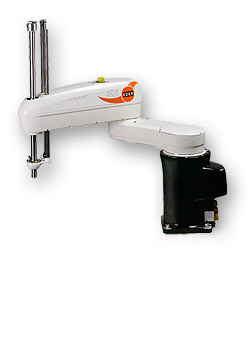
\includegraphics[scale=0.5]{./EtapaModerna/Imagenes/SCARA.jpg}
	\caption{SCARA (\href{https://commons.wikimedia.org/wiki/File:KUKA_Industrial_Robot_KR10_SCARA.jpg}{Wikimedia})}
	\label{fig:scara}
\end{figure}


%Inicios los movimientos humanos
\subsection{Mejora en la movilidad de los Robots}
\subsubsection{Introducción}

Tras el desarrollo de robots primigenios con funcionalidad concreta pero fija se planteó la posibilidad de integrar movimiento por el terreno en los mismos para poder realizar nuevas tareas u otras de forma más eficiente. En este ámbito se invirtió para lograr avances en esquivar objetos del escenario o en sistemas para andar basados en animales cuadrúpedos o bípedos como nosotros. A continuación analizamos de forma cronológica estos hechos.

\subsubsection{RB5X de RB Robot Corporation}
Un inicio en la movilidad en los robots fue incorporarles ruedas u orugas como herramientas para su desplazamiento por el suelo. Estos tipos de movimientos eran básicos, tales como hacia delante, hacia atrás o hacia los lados. Un avance en el movimiento inteligente lo protagonizó el Stanford's Cart, el cual fue progamado con sensores para desplazarse de una punta a otra de un recinto esquivando los objetos a su paso. Este movimiento inteligente era realizado gracias a un sistema de Visión por Computador que incluía el mismo. Tras esto surgieron nuevos intentos como el RB5X, un robot de pequeñas dimensiones capaz de desplazarse y evitar obstáculos o, en caso de no poder evitarlos, capaz de reconstruir su trayectoria tras impactar con algún objeto.

\vspace{10px}

El robot se ideó de forma multipropósito, puesto que los módulos que integraba eran programables por lo que las empresas tomaron el diseño y lo adecuaron a las tareas que se querían. El robot tuvo variantes tales como asistentes personales a los cuales les podías dar órdenes como recoger el periódico y a través de un brazo robótico que incluía poder interactuar con el medio. Además se le desarrolló una interfaz oral básica para poder darles las órdenes mediante la voz. Además era capaz de aprender de su entorno.

\subsubsection{Phony Pony}

Tras los intentos de hacer robots que incorporasen ruedas u orugas la Universidad de California del Sur realizó el desarrollo del que se conoce como primer robot cuadrúpedo llamado Phony Pony. El diseño de este robot se realizó en 1968 (anterior a RB5X) por los profesores e investigadores Frank y McGhee.

\vspace{10px}

El robot intentaba imitar las articulaciones de los animáles cuadrúpedos que conocemos de forma que lo desarrollaron con dos articulaciones: la cadera y la rodilla. De esta forma el robot podía mover la pierna hacia delante y además flexionarla. La velocidad del movimiento de las patas era extremadamente lenta, ya que al igual que ocurría con el Stanford Arm (contemporáneo a Phony Pony) los elementos eléctricos empleados en el movimiento estaban muy limitados. El Phony Pony era capaz de imitar comportamientos tales como andar, arrastrarse, agacharse o trotar.

\vspace{10px}

El control de este robot se realizaba de forma remota gracias a la tecnología desarrollada ya en esa época. Internamente el robot estaba diseñado mediante patrones de movimiento, de forma que estaba implementado con un autómata finito que tomaba las transiciones del mismo tras recibir la entrada del mando de control.

\subsubsection{WAP1}
En primer paso que se dió entorno a la idea de realizar un robot bípedo tuvo lugar en 1969 en la Universidad de Waseda en Japón. El robot WAP1 (Waseda's antropomorphic pneumatically-activated pedipulators) fue diseñado por el doctor Ichiro Kato.

\vspace{10px}

El doctor Ichiro Kato trabajaba por aquel momento en el terreno médico y empezó a intentar desarrollar músculos artificiales para poder sustituir músculos defectuosos en sus pacientes. El estudio desarrrolló una serie de dispositivos que al hincharse adquirían las formas que ellos necesitaban para simular el comportamiento de un músculo. Estas investigaciones darían sus frutos plasmándose en el primer robot bípedo creado. Los músculos que permitían el movimiento de WAP1 estaban hechos de goma y se inflaban con actuadores neumáticos. Este primer robot no era capaz más que de andar muy lentamente controlando el flujo de aire que se llevaba hacia las piezas de goma. Estas técnicas hacían que WAP llegara a tardar mucho tiempo en completar un paso, además de que no estaba pensado para andar una distancia dando pasos de forma consecutiva.

\vspace{10px}

En los dos siguientes años el doctor Ichiro Kato mejoró el diseño del WAP1 creado el WAP2 y el WAP3. La segunda versión de estos robots tuvo una mejora en la fuerza que los músculos eran capaces de aplicar sobre la estructura del mismo, pudiendo ahora levantar más peso y tener una estructura más robusta. La última versión fue desarrollada en 1971 y en esta el robot ya era capaz de rotar su movimiento, por lo que ya no tenían que ser movimientos rectos y, además, era capaz de superar pequeños obstáculos tales como ligeras inclinaciones o incluso escaleras de pequeño tamaño. Para poder desarrollar todo esto no sólo fueron necesarios los músculos artificiales del doctor Kato, si no además sus estudios en el control y mejora de la postura con lo que fueron capaces de controlar el centro de gravedad del robot, cosa completamente imprescindible para caminar sobre dos piernas.

\subsubsection{WL-9DR}
Tras los avances del doctor Ichiro Kato se intentó agilizar el movimiento de estos robots, puesto que el tiempo que había que esperar hasta que el WAP era capaz de avanzar un paso hacía que no fuera práctico su uso, ya que los robots que empleaban ruedas por ejemplo eran mucho más ágiles. Entre los años 1979 y 1980 la Universidad de Waseda desarrolló el WL-9DR bajo la dirección del doctor Kato, al igual que con sus predecesores los WAP.

\vspace{10px}

El funcionamiento de esta máquina también era mediante actuadores hidráulicos que operaban más rápidamente que los diseñados para WAP. Así mismo el control de este robot se hacía mediante un procesador de 16 bit conectado al robot mediante cables. El WL-9RD era capaz de dar un paso en 10 segundos, además de realizar ciclos completos andando, es decir, encadenar pasos para avanzar desde el punto de partida a un punto meta que se le fijaba. La velocidad con la que avanzaba era tan lenta que sus creadores no podían podían denominar al robot como dinámico, por lo que se le conoce como el primer robot bípedo cuasi-dinámico.

\vspace{10px}

El robot tenía un sistema de pesos que mantenía el equilibrio del mismo como se requiriera, por ejemplo si el robot estaba estático se centraba el punto de apoyo y se mantenía la postura tanto por la gran base rectangular de sus pies como por los pesos centrados. Si se quería dar un paso hacia delante el robot alzaba alguna de las piernas y se cambiaba el centro de los pesos un poco hacia delante, de forma que el robot se inclinara ligeramente para seguir con el siguiente paso. Para poder andar solamente 0.5 metros el robot requería sobre una docena de pasos llevándole entorno a un minuto completar dicha distancia.

\subsubsection{Aquarobot}
Tras los robots anteriormente mencionados (que sentaron precedentes en el tema de caminar) se siguieron desarrollando las técnicas que se empleaban en el equilibrio y las partes móviles de los mismos tal y como veremos en las siguientes secciones. Entre estos robots surgieron algunos proyectos que intentaron ir un poco más allá como el Aquarobot cuyo objetivo era ser capaz de andar bajo el agua.

\vspace{10px}

En el instituto de investigaciones de puertos de Japón se pensó en que sería útil que los operarios que tenían que trabajar bajo el agua dispusieran de facilidades para hacer la tarea más rápida y sencilla. Una de los trabajos que más tiempo llevaban en el puerto eran los de inspección bajo el agua para certificar el estado de las estructuras o diagnosticar algún tipo de fallo que se debía solventar. Por ello en el año 1984 se desarrolló la primera versión del Aquarobot, llegando a tener este hasta tres versiones diferentes haciendo mejoras sobre lo ya propuesto.

\vspace{10px}

El diseño básico del robot era una estructura con 6 patas capaz de andar bajo el agua. Los motores que empleaban eran de corriente continua (no neumáticos) colocados en cada una de las patas que iban selladas de forma estanca para impedir la entrada del agua. Además el robot era controlado por un pequeño procesador incluido en el mismo al que se le conectaban cables para comunicarlo con una computadora o un mando de control. El Aquarobot disponía asimismo de una cámara integrada que permitía ver en tiempo real lo que el robot observaba, de forma que los técnicos podían visualizar el estado del puerto sin necesidad de bajar ellos al agua.

\vspace{10px}

Cada pata tenía 3 grados de libertad con los que el robot podía andar y rotar sobre sí mismo. El peso aproximado de este robot era de unos 857 kilogramos en su primera versión y de unos 280 en la tercera. El sistema con el que se manipulaba al robot y los patrones de movimiento que se le definían en su propio procesador estaba programados en C++. El tiempo en el que el robot era capaz de responder a las órdenes que se le daban era de unos 50 milisegundos, gracias a la conexión que se tenía mediante cable.

\subsubsection{Honda y el gran avance}
La compañía Honda Motors, normalmente conocida por la fabricación de coches, tuvo un papel muy importante en el desarrollo de los robots antropomórficos y bípedos con sus series de robots, desde la serie E experimental, pasando por la P hasta los más que conocidos robots ASIMO que perduran actualmente.

\vspace{10px}

La serie de robots Honda E contó con 7 modelos, desde el 0 hasta el 6 desarrollados entre los años 1986 y 1993. Esta serie experimental comenzó en el mismo punto que el robot WAP, desarrollando un sistema que podía caminar sobre dos piernas. Estos robots, desde la versión 0, mejoraron enormemente los tiempos conseguidos por sus predecesores necesitando, ``únicamente'', 5 segundos para dar un paso completo. Este modelo contaba con 6 grados de libertad y con las articulaciones similares a las de una pierna humana, una cadera, la rodilla y el tobillo. En la versión 1 se mejoró la velocidad de movimiento pero se aumentó el peso haciéndo que fuera notablemente más grande que su versión anterior, además se le añadió un sistema mucho más complejo de articulaciones que le permitían tener 12 grados de libertad. En las versiones 2,3,4 y 5 se mejoró tanto el peso como la velocidad al andar, logrando que el robot anduviera de forma autónoma y dinámica llegando a los 4.7 kilómetros por hora. Cabe destacar que el diseño acabó con una cabeza muy grande y un peso de 150 kilogramos (comparados con los 16.5 de la versión 0). En la útltima versión no se modificó tanto el diseño y la velocidad al andar, si no que se centraron en que el robot fuera capaz de controlar el equilibrio de forma inteligente y fuese capaz de esquivar obstáculos e incluso no andar sobre un suelo liso.

\vspace{10px}

Tras el gran avance que lograron los ingenieros de Honda en cuanto a la capacidad de desplazamientos de la serie E, decidieron tomar todos esos avances y añadir más elementos para que pareciera cada vez más una persona. Tras la serie E vino la P con la intención de tomar lo obtenido de forma experimental en la anterior serie para continuar su camino hacia los robots antropomórficos. Estos robots fueron desarrollados entre los años 1993 y 2000. El primer modelo de la serie P supuso una transición en la cual se le añadieron brazos que, aunque no eran capaces de llevar una carga, le servían al robot para interactuar con el medio con acciones tales como abrir puertas o encender y apagar interruptores. En el modelo P2 Honda quiso marcar un precedente en la historia de la robótica haciendo que se pudiera desplazar andando, subir escaleras, empujar objetos e incluso llevar carga en las manos. El robot fue el primero en el que no se utilizaron cables para la comunicación con el mismo, para lo cual llevaba una batería incluida que permitía que trabajase alrededor de unos 15 minutos. La opinión pública se sorprendió enormemente, ya que este fue el primer robot conocido que tuvo un movimiento muy similar al humano. Tras el segundo modelo honda sacó el P3, cuyo objetivo con respecto a la versión anterior era reducir el peso, cosa que consiguieron ya que se pasó de 210 kilogramos a 130 sin variar las dimensiones del mismo más que en la profundidad del cuerpo del robot. El diseño además adquirió una semejanza mayor aún a los humanos con respecto al P2 y se mejoró la eficiencia de uso en la batería lo que permitió una autonomía de 25 minutos en lugar de los 15 minutos del P2. Por último se sacó el Honda P4, el que fue el último en la serie P de robots. Las dimensiones no variaron con respecto al P3 pero si el peso que se redujo a 80 kilogramos. Además este robot fue el que consiguió un movimiento más completo de la serie P con 34 grados de libertad contando brazos y piernas pero no se profundizó especialmente en esta versión puesto que los robots ASIMO estaban ya en desarrollo y Honda decidió acabar esta serie para dedicar todos sus esfuerzos en la nueva gama de robots.

\vspace{10px}

La serie de robots ASIMO o (Advanced Step in Innovative Mobility) fueron la continuación de la serie P de Honda en cuanto a la creación de un robot humanoide. Los robots ASIMO tuvieron diferentes revisiones, esta vez no divididas en diferentes versiones. La primera versión se sacó a la luz en el año 2000 para después tener nuevas mejoras en los años 2002, 2005, 2007 y 2011. Los ASIMO comenzaron teniendo una altura de 120 centímetros y 54 kilogramos de peso, un gran avance comparando los pesos y alturas con los obtenidos en la serie P que llegaban a pesar 210 kilogramos. ASIMO mejoró en la velocidad en la que andaba pasando de 1.6 kilómetros por hora a 2.7 kilómetros por hora. En sus primeros modelos ASIMO no era capaz de correr pero en el modelo de 2004 la funcionalidad se añadió comenzando a correr a 3 kilómetros por hora hasta los 9 de la versión de 2011. La batería que incorporaban los Honda P fue reutilizada en las primeras versiones de los ASIMO pero ésta cambió a una batería de ión de litio desde el 2004 para llegar a dar una hora completa de batería en uso mixto (andando y corriendo). Además los grados de libertad que obtuvo la versión de 2011 fueron 57, un número muy superior a los 26 del modelo del año 2000 que permitía movimientos no sólo de brazos y piernas si no también movimientos completos de los dedos de la mano con lo que la última versión es capaz de hacer gestos con la misma y movimientos complejos parecidos a los que podemos realizar con nuestra mano. Además en la última versión se le añadió un sistema de voz con el que las personas nos podemos comunicar con ASIMO para pedirle tareas específicas. En su última versión el robot ASIMO es capaz de reconocer el entorno que le rodea mediante cámaras y sensores de visión incorporados en su casco con los cuales ASIMO no sólo es capaz de interactuar con las personas por voz, si no que también es capaz de analizar los movimientos y comportamientos de las mismas para actuar en función de ello. Además en cuanto a la interfaz oral no sólo responde mediante altavoces para continuar la conversación, si no que además también gesticula para dar una interacción más humana.

Con los robots ASIMO Honda completó una era en cuanto a los movimientos en la robótica al conseguir un movimiento al caminar natural y rápido y una interacción con el medio a través de las manos y brazos muy extensa. Tras esto los robots antropomórficos han seguido avanzando pero todos utilizando en gran medida la senda que Honda marcó con su series E, P y ASIMO.


%iRobot
\subsection{iRobot}
En el camino de la creación de robots hasta este momento se habían diseñado pensando siempre en su aplicación empresarial o industrial. ASIMO pudo ser el primero en el que la gente se pudiera replantear su utilidad dentro de una casa para cumplir tareas sencillas, pero debido a su alto precio (incluso no fueron comercializados más allá de hacer demostraciones para empresas) no eran accesibles a nadie o casi nadie. En este punto surgió la compañía iRobot Corporation, una compañía fundada por tres ingenieros del MIT: Rodney Brooks, Colin Angle y Helen Greiner quienes venían de trabajar y estudiar en el Laboratorio de Inteligencia Artificial del MIT.

iRobot cambió un poco la perspectiva de las personas al hacer que se incluyeran en casa robots de un precio asequible cuyas aplicaciones reales eran verdaderamente útiles (no como un asistente ASIMO en una casa).

La compaía fue fundada en 1990, época por la cual trabajaban con robots aplicados a la tecnología militar, como fue su robot PackBot usado en las guerra de Iraq y Afghanistan como apoyo a las tropas. El robot era útil puesto que incorporaba un sistema que le permitía superar obstáculos tales como piedras, escaleras, huecos, etc gracias a las orugas con las que se desplazaba. iRobot además no sólo tuvo contratos con la industria militar si no que, además, mantuvo relaciones con la NASA desarrollando robots para ellos también.

Tras los contratos mencionados anteriormente iRobot comenzó su andadura en los robots de ámbito doméstico con robots dedicados a la limpieza y archiconocidos: los Roomba, Braava y Mirra. De aquí los más conocidos son los del modelo Roomba. Este robot actualmente es capaz de barrer y fregar una casa de forma autónoma y aunque nos parezca trivial o de poca relevancia no lo es en absoluto. Estos robots incorporan todo el desarrollo de los mencionados anteriormente, no sólo la capacidad de moverse y limpiar, si no también la capacidad de aprender de su entorno haciendo un mapa de las habitaciones, ser capaz de esquivar obstáculos y recalcular su trayectoria, así como la capacidad de volver al punto de donde partió (su base de carga). Este modelo en concreto es un hito en la historia de la robótica al traer a casa tecnología muy avanzada en cuestión de robótica y domótica a un precio más asequible que los robots diseñados hasta el momento.


%Estado actual de la robótica
\subsection{State of Art de la Robótica}
Hasta ahora hemos visto cómo la robótica dió sus primeros pasos tras la concepción de los laboratorios de Inteligencia Artificial por todo el mundo, con lo que se produjo un boom en las técnicas y el desarrollo de la robótica. No se le escapará a nadie que actualmente a la cabeza de la robótica podemos encontrar ciertas secciones o categorías que se están desarrollando por encima del resto ya sea por su utilidad, por lo vistosos que son o por el simple hecho de buscar un desarrollo en dicho campo. Estas categorías podrían ser: los robots usados en el espacio o expediciones espaciales, los robots usados en la industria militar, los robots diseñados mediante la IA para algún tipo de tarea concreta o los robots que imitan cualidades humanas.

A continuación trataremos de discutir el actual estado de los robots en estas categorías.

\subsubsection{NASA}
Dentro del panorama aeroespacial la agencia que lidera actualmente el desarrollo en la exploración fuera de la Tierra es la NASA. Gracias a esto la agencia espacial estadounidense ha desarrollado un programa de robótica muy amplio y robusto, con robots que van desde la asistencia en viajes espaciales hasta exploración del espacio, telescopios o robots usados en exploraciones planetarias.

Entre los robots diseñados por la NASA no sólo hay robots pensados para la exploración de planetas, también se han ideados robots de asistencia para los astronautas. En este grupo de robots podemos meter a la serie Robonaut con las dos versiones desarrolladas hasta el momento. Esta gama de robots están pensados para la asistencia tanto dentro de la nave espacial como fuera de la misma, por ejemplo en tareas de reparación o acoplamiento de módulos. El primer modelo, el Robonaut 1 o R1 nunca llegó al espacio, si no se que empleó como un primer prototipo para estudio y desarrollo. El robot consistía de un torso con forma humana y con la parte de abajo intercambiable, de esta forma se podía adecuar el mismo para la exploración de planetas o colocarle módulos como el Zero-G Leg, pensado para poder engancharse a las barras exteriores que se le suelen colocar a los módulos, naves y estaciones espaciales para facilitar el desplazamiento de los astronautas por el exterior de las mismas (en esta misma línea la NASA tiene un concepto de robot llamado Spidernaut). De esta manera se demostraba que este robot, si se diseñara de forma adecuada, sería útil en misiones de reparación en el exterior de las naves o de asistencia. En su segunda versión el robot mejoró todas sus capacidades y el diseño se convirtió realmente en algo funcional siendo lanzado en 2011 a la ISS (Estación Espacial Internacional). El primer modelo que se envió a la estación no era capaz de moverse pero sí de llevar cosas y mover sus brazos de forma que era útil para sostener cosas como herramientas o moverlas de un sitio a otro con la rotación del torso. Tras ese paso se enviaron a la ISS piernas y módulos extra al robot de forma que ahora ya es capaz de moverse dentro de la estación y es capaz de ver y analizar su entorno. Por el momento no se ha conseguido presurizar el cuerpo lo suficiente como para poder emplearlo en misiones fuera de la estación. Actualmente esta es la línea de desarrollo del robot tanto para misiones fuera de la estación como para misiones de exploración del espacio profundo.

En este mismo sentido la compañía canadiense MDA, en su aportación a la ISS, diseñó el robot Dextre con una funcionalidad muy parecida a la ideada para Robonaut. El robot consiste de un cuerpo de enormes dimensiones con dos brazos robóticos capaces de moverse muy rápido. El objetivo de este robot es que sea capaz de realizar tareas para las que antes se requería la salida de alguno de los astronautas de la ISS al exterior de la misma. Este hecho se ha conseguido de tal forma que ni siquiera se tiene por qué operar desde la ISS, si no que se puede realizar el manejo del mismo desde la Tierra. De esta forma, tal y como ocurrió en su primera misión, se pueden realizar tareas de mantenimiento sin necesidad de que los miembros de la ISS estén disponibles o incluso aunque estos estén dormidos. El robot tiene un cuerpo que mide unos 3.5 metros de longitus y dos brazos de 3.5 metros cada uno pesando en total más de 1600 kilogramos.

La NASA también tiene robots que aún no han sido empleados en misiones reales pero sí se sigue avanzando en su desarrollo, como es el caso del RASSOR (Regolith Advanced Surface Systems Operations Robot). Este robot está diseñado para operaciones de construcción y alisamiento del terrreno, extracción de agua, eliminar el hielo de una zona concreta, retirar arena, etc. El RASSOR actualmente está en fase de pruebas, pero se le espera un buen futuro por su mínimo coste de producción y por la versatilidad del mismo, puesto que sería capaz de trabajar unas 16 horas por día durante muchos años. El robot además, por su diseño, está pensado para superar los obstáculos que se le presenten y para poder corregir su posición incluso si vuelca. Para las tareas que se planean que pueda realizar el robot incorpora dos ruedas como las de una trituradora industrial (una en la parte delantera y otra en la trasera) capaces de ser movidas de forma independiente.


\normalsize


% Bibliografía.
%-----------------------------------------------------------------
\onecolumn
\bibliography{EtapaModerna}
\bibliographystyle{plain}
\nocite{*}

\end{document}
